%% ==================================================================
%% Home version - 03-Jan: 19:26 pm
%% ==================================================================

\documentclass[referee, sn-mathphys-num]{sn-jnl}
\bibliographystyle{unsrt}
%\bibliography{bibliography}

%%%% Standard Packages
%% <additional latex packages if required can be included here>
\usepackage{subfigure}% Support for small, `sub' figures and tables
\usepackage{chronosys} 	% Chronology
\usepackage{xcolor, soul, colortbl} % Highlights
%\usepackage{algorithm}
%\usepackage[noend]{algpseudocode}
%\usepackage{booktabs}	% Tables
\usepackage{arydshln} 	% dashed lines in tables
%\usepackage{multirow}	

%\usepackage[spaces, hyphens]{url}
%\usepackage[colorlinks, allcolors=black]{hyperref}
%\usepackage[colorlinks, allcolors=blue]{hyperref}
%%  <additional latex packages if required can be included here>

\usepackage{graphicx}%
\usepackage{multirow}%
\usepackage{makecell}%
\usepackage{amsmath,amssymb,amsfonts}%
\usepackage{amsthm}%
\usepackage{mathrsfs}%
\usepackage[title]{appendix}%
% $$ \usepackage{xcolor}%
\usepackage{textcomp}%
\usepackage{manyfoot}%
\usepackage{booktabs}%
\usepackage{algorithm}%
\usepackage{algorithmicx}%
\usepackage{algpseudocode}%
\usepackage{listings}%
%%%%

\raggedbottom
%%\unnumbered% uncomment this for unnumbered level heads

% Macros
\algnewcommand{\LineComment}[1]{\State \(\triangleright\) #1}
\newcolumntype{L}[1]{>{\raggedright\let\newline\\\arraybackslash\hspace{0pt}}p{#1}}
\newcolumntype{C}[1]{>{\centering\let\newline\\\arraybackslash\hspace{0pt}}p{#1}}
\newcolumntype{R}[1]{>{\raggedleft\let\newline\\\arraybackslash\hspace{0pt}}p{#1}}
\newcommand{\rowspace}[1]{\renewcommand{\arraystretch}{#1}}
\newcommand{\ltmidrule} {\arrayrulecolor{black!20} \midrule}
\newcommand{\drmidrule} {\arrayrulecolor{black!40} \midrule}
\newgeometry{left=1in, top=1in, right=1in, bottom=1in}

\definecolor{codegray}{rgb}{0.5,0.5,0.5}
\definecolor{ltgray}{gray}{0.93}
\definecolor{dblue}{rgb}{0.20, 0.30, 1.0}

\newcommand{\hlc}[2][cyan!15]{{\colorlet{foo}{#1}\sethlcolor{foo}\hl{#2}}}
\makeatletter
\def\SOUL@hlpreamble{%
	\setul{}{2.8ex}% default is 2.5ex
	\let\SOUL@stcolor\SOUL@hlcolor
	\SOUL@stpreamble
}
\makeatother

\begin{document}
	
	\title[REINFORCE for Predictive Maintenance]{An Empirical Study of the Na\"ive REINFORCE Algorithm for Predictive Maintenance}
	
	\author[1,4]{\fnm{Rajesh} \sur{Siraskar} \sfx{(\href{https://orcid.org/0000-0003-2341-8787}{ORCID: 0000-0003-2341-8787}})}\email{rajesh.siraskar@gmail.com}
	\author*[1,2]{\fnm{Satish} \sur{Kumar}}\email{satish.kumar@sitpune.edu.in}
	\author[1,2]{\fnm{Shruti} \sur{Patil}}
	\author[1]{\fnm{Arunkumar} \sur{Bongale}}
	\author[1,2]{\fnm{Ketan} \sur{Kotecha}}
	\author[3]{Ambarish Kulkarni}
	
	\affil*[1]{\orgdiv{Symbiosis Institute of Technology}, \orgname{Symbiosis International (Deemed University)}, \orgaddress{\city{Pune}, \postcode{412115}, \state{Maharashtra}, \country{India}}}
	\affil[2]{\orgdiv{Symbiosis Centre for Applied Artificial Intelligence}, \orgname{Symbiosis International (Deemed University)}, \orgaddress{\city{Pune}, \postcode{412115}, \state{Maharashtra}, \country{India}}}
	\affil[3]{Swinburne University of Technology, Hawthorn VIC 3122, Australia}
	\affil[4]{\orgdiv{CTO Office}, \orgname{Birlasoft Ltd.}, \orgaddress{\city{Pune}, \postcode{411057}, \state{Maharashtra}, \country{India}}}
	
	\abstract{
		Reinforcement Learning (RL) is a biologically inspired, autonomous (self-learning) machine learning (ML) method. RL algorithms can help generate optimal predictive maintenance (PdM) policies for complex industrial systems. However, these algorithms are extremely sensitive to hyperparameter tuning and network architecture, and this is where automated RL frameworks (AutoRL) can offer a platform to encourage industrial practitioners to apply RL to their problems. AutoRL applied to PdM has yet to be studied. Aimed at practitioners unfamiliar with complex RL tuning, we undertake an empirical study to understand \textit{untuned} RL algorithms for generating optimal tool replacement policies for milling machines.
		
		\textcolor{red}{\hlc{contribution --- MENTION SENSITIVITY ANALYSIS OF HPs on this domain is NOT done}}
		
		We compare a na\"ive implementation of REINFORCE against the policies of industry-grade implementations of three advanced algorithms -- Deep Q-Network (DQN), Advantage Actor-Critic (A2C), and Proximal Policy Optimization (PPO). Our broad goal was to study model performance under four scenarios: (1) simulated tool-wear data, (2) actual tool-wear data (benchmark IEEE\textit{DataPort} PHM Society datasets), (3) univariate state with added noise levels and a random chance of break-down, and finally (4) complex multivariate state. Across 15 environment variants, REINFORCE models demonstrated higher tool replacement precision and F1 of 0.687/0.609 against 0.449/0.442 for A2C, 0.418/0.374 for DQN, and 0.472/0.345 for PPO, while demonstrating lower variability. Comparing the best \textit{auto-selected} model, over ten training rounds produced unusually wider performance gaps with the REINFORCE precision/F1 at 0.884/0.873. The best A2C, DQN, and PPO models produced 0.520/0.639, 0.651/0.740, and 0.558/0.580, respectively. Our findings, surprisingly, indicate that the computationally lightweight REINFORCE performs significantly well for this particular problem and forms a small step toward AutoRL for PdM.}	
	\keywords{Reinforcement Learning, predictive maintenance, REINFORCE}
	
	\maketitle
	
	\section*{\hlc{Article Highlights}}
	\begin{enumerate}
		\item \hlc{Contributes to the broader goal of AutoRL (Automated Reinforcement Learning) for Predictive Maintenance}
		\item \hlc{Research for practitioners with limited hyperparameter tuning expertise -- focusing on practical industry needs}
		\item \hlc{REINFORCE, despite computational simplicity, outperforms complex algorithms under default configurations}
	\end{enumerate}
	
	\section{Introduction}
	%% Quote
	%\epigraph{"Plurality should not be posited without necessity" -- Of two competing theories, the simpler explanation of an entity is to be preferred}{--- \textup{William of Ockham (1285?1347)}, The Occams razor principle}
	%% End Quote and first line of para without indent
	
	Milling machines are highly versatile, ubiquitous tools serving a variety of industries. A milling machine removes metal from the work piece by rotating and driving a cutting device into it. Abrasive forces cause tool wear, and optimal tool replacement reduces direct costs and optimizes the machines' downtime. This is an important goal, considering that the global milling machine market is valued at USD 68.3 billion \cite{milling-market}. The cutting tool experiences multiple types of wear as it cuts through metal. Tool wear depends on several factors such as the cutting speed, force applied to the tool, lubrication and materials of the work piece and cutting tool. 
	
	Reinforcement learning (RL) is an artificial intelligence technique inspired by nature. Of all the foundational machine learning (ML) methods, RL is the closest method of learning as seen in animals and humans. Biological learning systems use the learning feedback loop, Fig. \ref{fig_RL-loop}, that inspired core RL algorithms, \cite{barto2018}.
	
	An actor or ``agent'' interacts with an environment and learns via ``trial-and-error''. It acts based on stimuli or feedback received from the environment after performing a certain action. Actions that help in achieving the learning goal receive a reward while actions that do not, are punished. Repeating this loop over thousands of episodes ``reinforces'' good actions thereby building a ``policy'' that is optimized for that goal. In the case of predictive maintenance for milling machines, the agent is the ``planner'' with a goal of learning an optimal tool replacement policy. The environment is technically anything other than the agent -- sensors attached to the machine, job specifications, ambient conditions etc.
	\begin{figure}[h]
		\centering
		\includegraphics[width=0.5\textwidth]{RL-loop.pdf}
		\caption{Reinforcement Learning, \cite{barto2018}}
		\label{fig_RL-loop}
	\end{figure}
	
	AutoML offers automated machine learning (ML) platforms. Once the user feeds in data and sets an objective, they detect data types of features and response variables, select suitable ML techniques from a library, run techniques like grid-search on the hyperparameter space, train the models, select evaluation metrics, evaluate the models using techniques such as hold-out or cross-validation and finally select the best model. Such automated pipelines are often available for supervised and unsupervised ML fields. AutoML for RL, called AutoRL, is conceptually similar and intended for automating RL development. However RL is extremely sensitive to hyperparameter and network architectures and this prevents practical out-of-the-box use of RL, \cite{autorl:shala2022, autorl:afshar2022}. Successful RL agents must therefore be manually trained by experts \cite{autorl:parker2022}, which unfortunately \hlc{restricts the application} of these learning methods across the wide industrial domain.
	
	\begin{figure}[hbt!]	
		\startchronology[startyear=1940, startdate=false, stopdate=false, arrow=false, color=codegray, height=.5ex]
		\chronoevent[textwidth=2.25cm]{1947}{Monte Carlo\endgraf \texttt{    }sampling}
		\chronoevent[markdepth=-20pt]{1959}{TD Learning}
		\chronoevent{1989}{Q-Learning}
		\chronoevent[markdepth=-20pt]{1992}{\textcolor{blue}{REINFORCE}}
		\chronoevent{2013}{DQN}
		\chronoevent[markdepth=-20pt]{2016}{A2C}
		\chronoevent[markdepth=50pt]{2017}{PPO}
		\stopchronology
		\vspace{-36pt}
		\caption{Time line of significant RL algorithms}
		\label{fig_TimeLine}
	\end{figure}
	Introduced in 1992, the REINFORCE algorithm \cite{REINFORCE-williams1992} is an early policy based RL algorithm, capable of handling both discrete and continuous observation and action spaces. In practice the REINFORCE algorithm is considered a ``weak'' algorithm and superseded by several algorithms developed since. Most notably the deep-neural network version of Q-Learning, the Deep Q-Network (DQN) \cite{DQN-mnih2013}, followed by Actor-Critic \cite{A2C-mnih2016} and one of the most robust modern-day algorithms, the Proximal Policy Optimization (PPO) \cite{PPO-schulman2017}, Fig. \ref{fig_TimeLine}. Our study takes a fresh look at REINFORCE, an otherwise neglected algorithm comparing it against three advanced algorithms, namely, DQN, Advantage Actor-Critic (A2C), and PPO. Secondly, while most RL studies are evaluated on OpenAI Gym environments, our experiments cover the PdM problem using a custom built environment. In practice the milling tool is replaced after a set threshold. We use this ``deterministic preventive maintenance'' policy as the baseline for comparing the various policies. Our systematic evaluation, based on levels of environment difficulty, different bench-mark datasets and varying noise levels allow a broader comparison of the algorithms. Finally, we conduct statistical tests to ensure a robust statistical-evidence based conclusion.\\
	
	The main contributions of this research are:
	\begin{enumerate}
		\item Contributes to the broader goal of AutoRL for predictive maintenance.
		\item Targeted toward industrial practitioners not accustomed to RL hyperparameter tuning.
		\item Design and implement an RL environment for predictive maintenance of a milling machine.
		\item Rigorous evaluation of four standard, untuned, RL algorithms.
		\item \hlc{Research focus on the computationally light REINFORCE algorithm.}
		\item Use of simple performance evaluation statistical measures and plots that industrial practitioners are normally used to.
	\end{enumerate} 
	
	The rest of the paper is structured as follows: In the next section we survey some related work and provide the necessary technical background describing the algorithms studied in this research. Sec. \ref{sec_Method} discusses implementation details of the REINFORCE algorithm and the PdM environment followed by the methodology adopted for training, testing and evaluation. Sec. \ref{sec_Results} and \ref{sec_Discussion} present and discuss, the results of experiments. Finally, we summarize and draw conclusions in Sec. \ref{sec_Conclusion}.
	
	\section{Related work and background}\label{sec_SLR}
	In this section we survey the intersection of past work related to RL for PdM, specifically milling machines and AutoRL.
	
	\subsection{Literature Review}
	\hlc{We reviewed related research to establish research gaps that we could address. Our work is meant to assist practitioners apply RL for predictive maintenance. It touches the dual fields of HPO (hyperparameter optimization) and the development of the AutoRL.} 
	
	Application of RL for PdM has been surveyed by \cite{Panzer2021, Erhan2021, siraskar2023}. \hlc{There are no research articles that cover AutoRL for predictive maintenance. We therefore widened our scope and searched for AutoML for PdM resulting in 21 articles, of which 14 were conference papers and 7 published in journals, Fig. {\ref{fig_artcilestats}}, however the research coverage remained limited to supervised ML and excluded RL and AutoRL.}\footnote{As of: 21-Dec-2024, across IEEE Xplore\texttrademark{}, Scopus\texttrademark{} and Web Of Science\texttrademark{}}.
	% trim=left botm right top. % \fbox{\includegraphics[trim=3.5cm 18.75cm 4cm 3.3cm]{articlestats.pdf}}
	\begin{figure}[hbt!]
		\centering
		\includegraphics[width=0.4\textwidth, trim={3.5cm 18.25cm 4cm 3.3cm}]{articlestats.pdf}
		\caption{\hlc{Research articles related to AutoML and PdM. None were found on AutoRL for PdM.}}
		\label{fig_artcilestats}
	\end{figure} 
	
	Experimental comparison of RL algorithms, has been limited to using standard benchmark OpenAI Gym environments: \cite{sandeep2022experimental} documents experimental evaluation of four policy-gradient and actor-critic algorithms PPO, Soft Actor Critic (SAC), Deep Deterministic Policy Gradient (DDPG) and A2C using the Pendulum, Mountain Car, Bipedal Walker, Lunar Landing and Atari 2600 game environments. \cite{Krishna2020} evaluate DQN, DoubleDQN, A2C, REINFORCE and PPO using Cartpole, Space Invaders and the Lunar Lander. \cite{dulac2021, dulac2020empirical} are significant contributions toward analyzing \textit{real-world} challenges. They performed empirical studies on Cartpole, humanoid and walker environments\footnote{From the Real-World Reinforcement Learning (RWRL) Suite} by embedding them with real-world design concepts and then evaluating REINFORCE, Trust Region Policy Optimization (TRPO) and DDPG.
	
	\cite{dulac2021, henderson2018deep} evaluate RL for continuous control. \cite{henderson2018deep} study DDPG, ACKTR, TRPO and PPO, using, like we do, the OpenAI RL implementations, on complex MuJoCo\footnote{\href{https://mujoco.org/}{MuJoCo}: `Multi-Joint dynamics with Contact' e.g. HalfCheetah, Hopper, Walker and Swimmer} environments. \cite{ford2022cognitive} is one experimental evaluation we found covering a \textit{real-world} application where DQN, A2C and PPO are applied for choosing the operational radio frequency (RF) mode for a multi-function RF system and go on to recommend PPO as the best.
	
	%% Connecting AutoRl + HPO
	\hlc{None of the AutoRL articles covered PdM, we therefore study them for their contribution toward creating AutoRL frameworks in general}. \cite{autorl:parker2022} \hlc{is a detailed technical assessment and survey of the AutoRL field. They provide a deep dive into the techniques and methods to automate the RL training pipeline, outline the implied challenges and the open research questions that remain. They observe that it is the methods that can \textit{dynamically adapt hyperparameter} configurations during the training cycle that will generate the best models; however their study concluded that, despite substantial research, it is not yet clear which hyperparameters must be optimized dynamically and which statically. A second important conclusion was the acknowledgment that relation of hyperparameters to environments was as yet undetermined. They align with} \cite{Eimer2023AutoRL}, \hlc{that hyperparameter optimization will vary and be \textit{specific to an environment}}. 
	
	\cite{autorl:shala2022} \hlc{are the first to propose a \textit{tabular AutoRL benchmark} for studying the hyperparameters of RL algorithms. They have considered hyperparameter search spaces for five RL methods - PPO, DDPG, A2C, SAC and TD3, across 22 OpenGym, environments. They studied four hyperparameters of which only two were common across all five algorithms -- the learning rate and discount factor {$\gamma$}. They did not address any network design hyperparameter.}
	
	\hlc{The main contribution of} \cite{autorl:afshar2022} \hlc{is the proposition of a \textit{generalized AutoRL framework} split into three main components -- MDP (Markov Decision Process) modeling, algorithm selection and hyperparameter optimization.}
	
	\hlc{All AutoRL related work} \cite{autorl:afshar2022, autorl:parker2022, autorl:shala2022, Eimer2023AutoRL}, \hlc{point unanimously toward three research gaps: First, unlike AutoML pipelines, AutoRL as a usable framework has not yet been developed, second there is no ideal hyperparameter configuration setup that is clearly optimal for all or even a set of related environments, and third domain specific work is required for AutoRL to be effective in solving real world problems.} 
	
	\hlc{The authoritative{\footnote{A collaborative research effort between universities Oxford, Leibniz, Freiburg and organizations Google, Meta and Amazon}} work by} \cite{autorl:parker2022} \hlc{mention that as a completely closed-loop system, in RL, each of its component influences the other. This therefore poses a challenge for automatic tuning as any interim system evaluation (during training) is highly likely to be stochastic due to the interaction of various noise sources (e.g. policy, environment). They concluded that no AutoRL approach has been developed to offer the best combination of an algorithm itself and then its configuration}. 
	
	%% LR consolidate
	\hlc{The literature survey helped identify the following open areas and helpful pointers for our research:}
	\begin{enumerate}
		\item \hlc{\textbf{Predictive maintenance} is an unexplored domain. Build a predictive maintenance RL environment and train an agent for taking maintenance actions.}
		\item \hlc{The \textbf{REINFORCE} algorithm has not been studied and evaluated within a PdM environment.}
		\item \hlc{A comparison of \textbf{untuned} RL methods may enhance our understanding of how best to create automated techniques to address the interaction between algorithm and hyperparameter settings.}
		\item \hlc{A good selection of \textbf{common hyperparameters} across the algorithms are the learning rate and discount factor {$\gamma$}.}
		\item \hlc{None of the AutoRL comparative studies covered network architecture elements - consider covering at least one important \textbf{network hyperparameter}}.
	\end{enumerate}
	
	\hlc{Our work focuses on RL. Supervised machine learning can be used to solve such problems i.e. detect when the fault part needs replacement. As a final part of this existing literature study, we briefly table related ML work in Table {\ref{tbl_ml}} that we can compare to, later in the Discussion Sec. {\ref{sec_Discussion}}}
	
	\begin{table}[hbtp!]
		\rowspace{1.5}
		\caption{\hlc{ML based solutions for similar predictive maintenance problem.}}%\label{tab1}%
		{\begin{tabular}[h]{L{4cm} L{4cm} L{2.75cm} R{1.25cm} L{3cm}}
				\arrayrulecolor{black!40}\toprule
				\hlc{ML technique} & \hlc{Time series} & \hlc{Research article} & \hlc{Accuracy} & \hlc{Domain - use-case} \\
				\midrule	
				Support Vector Machine & Time domain, multivariate & \citeauthor{niu2020-93ML} \cite{niu2020-93ML} & 0.967 & \multirow{8}{3cm}{Milling tool-wear condition monitoring}\\
				k-Nearest Neighbour & Time-domain with wavelet transforms & \citeauthor{yang2020-94ML} \cite{yang2020-94ML} & 0.948 & \\
				Support Vector Machine & Time-domain with wavelet transforms & \citeauthor{lei2020-95ML} \cite{lei2020-95ML} & 0.908 & \\
				Support Vector Machine & Time and frequency domain & \citeauthor{zhou2020-96ML} \cite{zhou2020-96ML} & 0.908 & \\
				Support Vector Machine & Time domain, multivariate & \citeauthor{ou2020-97ML} \cite{ou2020-97ML} & 0.918 & \\
				Naive Bayes and k-Star & Time domain, multivariate & \citeauthor{madhusudana2016-64ML} \cite{madhusudana2016-64ML} & 0.969 & \\
				Tree family classifiers & Time domain, multivariate & \citeauthor{patange2019-23ML} \cite{patange2019-23ML} & 0.890 & \\
				Calibration model (reference signal based) & Time domain, multivariate & \citeauthor{liu2020-92ML} \cite{liu2020-92ML} & 0.900 & \\ \midrule
				CNN with Attention Knowledge Distillation & Time domain, multivariate & \citeauthor{fu2023ML} \cite{fu2023ML} & 0.972 & \multirow{2}{3cm}{Bearings: Classification of faults}\\
				CNN based LeNet & Time domain, multivariate & \citeauthor{pandey2023ML} \cite{pandey2023ML} & 0.953 & \\ \midrule
				Nadaraya-Watson Attention mechanism & Time domain, univariate & \citeauthor{Siraskar2024ML} \cite{Siraskar2024ML} & 0.984 & \multirow{2}{3.5cm}{Milling tool-wear fault detection. Performance in $R^2$}\\
				Nadaraya-Watson Attention mechanism & Time domain, multivariate & \citeauthor{Siraskar2024ML} \cite{Siraskar2024ML} & 0.834 & \\
				
				\bottomrule
		\end{tabular}}
		%\footnotetext[-]{Note: ``NA'' implies not-available or not-applicable.}
		\label{tbl_ml}
	\end{table}	
	
	\subsection{Technical Background}
	\subsubsection*{Key concepts of RL}
	A task is a goal we set for our agent to learn. In our case the agent must learn to optimally predict the replacement of the tool. Frequent tool replacements increases down-time while delaying it results in inferior work piece quality. In Fig. \ref{fig_RL-loop} the agent interacts with the environment by performing an action ($a \in \mathcal{A}$), which then alters the state of the environment to one of many states ($s \in \mathcal{S}$). The resulting state is determined by state-transition probabilities ($\mathcal{P}$) as governed by Markov Decision Process (MDP) theory. The new state provides a feedback via a reward ($r \in \mathcal{R}$). Higher positive rewards ``reinforce'' good behavior. Performing this over thousands of episodes with the objective of maximizing the total rewards $R$, enables the agent to develop a policy $\pi$ which is essentially a mapping of the optimal action to perform given a certain state.
	
	A \textbf{value function} computes how good a state or an action is by predicting future rewards, also known as a ``return'' $G_t = R_{t+1} + \gamma R_{t+2} + \dots = \sum_{k=0}^{\infty} \gamma^k R_{t+k+1}$. $\gamma \in [0, 1]$ facilitates discounting i.e. applying less weight to future rewards. Value functions can be represented by \textbf{state-value} $V_{\pi}(s)$ of a state $s$, as the expected return: $V_{\pi}(s) = \mathbb{E}_{\pi}[G_t \vert S_t = s]$; or an \textbf{action-value} function of a state-action pair as $Q_{\pi}(s, a) = \mathbb{E}_{\pi}[G_t \vert S_t = s, A_t = a]$.
	
	With this brief overview of RL, we look at the core ideas of the four algorithms we experimented with.
	
	\subsubsection*{Deep Q-Network (DQN)}
	Deep Q-Network \cite{DQN-mnih2013} significantly improved the earliest RL algorithm, Q-learning, by introducing neural networks to learn policies for high-dimension environments with two novel strategies to significantly stabilize learning -- an ``experience replay buffer'' and a target network that was frozen and only periodically updated. Equation \eqref{eq_DQN} shows the DQN loss function where $D$ is the replay memory, sampled using a uniform distribution $U(D)$, $Q(s, a; \theta)$ parameterized with $\theta$, helps compute the Q values and $\theta^{-}$ represents parameters of the frozen target Q-network. The objective then is to minimize this loss.
	
	\begin{equation}\label{eq_DQN}
		\mathcal{L}(\theta) = \mathbb{E}_{(s, a, r, s') \sim U(D)} \Big[ \big( r + \gamma \max_{a'} Q(s', a'; \theta^{-}) - Q(s, a; \theta) \big)^2 \Big]
	\end{equation}
	
	\subsubsection*{Advantage Actor Critic (A2C)}
	
	A2C is a variant of Asynchronous Advantage Actor Critic (A3C) \cite{A2C-mnih2016}, and uses multiple computation workers to avoid the use of a replay buffer. A2C is a policy-gradient actor-critic algorithm. Policy-gradient algorithms strive to model and optimize the policy directly. Actor-critic structures consist of two networks -- a critic that updates function parameters $w$ of the value function (i.e either $Q_w(a \vert s)$ or $V_w(s)$); and an actor that updates the policy parameters $\theta$ for $\pi_\theta(a \vert s)$, following the direction computed by critic. Actors therefore learn the parameterized policy $\pi_{\theta}$ using the policy-gradient as shown in (\ref{eq_A2C}). 
	\begin{equation}\label{eq_A2C}
		\nabla_ \theta J(\pi_\theta) = \mathbb{E}_t \; [ \; A^\pi_t \; \nabla_\theta \ln \pi_\theta(a_t \vert s_t) \;]
	\end{equation}
	Where the advantage function $A^\pi_t (s_t, a_t)$ measures how good or bad the action is w.r.t. policy's average, for a particular state, using (\ref{eq_A2CAF}).
	\begin{equation}\label{eq_A2CAF}
		A^\pi_t (s_t, a_t) = Q^\pi (s_t, a_t) - V^\pi (s_t)
	\end{equation}
	
	\subsubsection*{Proximal Policy Optimization (PPO)} 
	\cite{PPO-schulman2017} formulated PPO which is often considered as the most robust of the RL algorithms. PPO is a policy-gradient method based on TRPO (Trust Region Policy Optimization) by \cite{TRPO-schulman2015}, where the core idea is the use of a trust region to improve training stability by avoiding updates to parameters that vastly change the policy at a particular time step. TRPO ensures this by using a divergence constraint on the magnitude of policy update. If $r(\theta)$ (\ref{eq_rPPO}) represents the ratio of probabilities between policies of previous and current iteration, then the objective function of TRPO is given by (\ref{eq_TRPO}), where $\hat{A}$ represents the estimated advantage function.
	\begin{equation}\label{eq_rPPO}
		r(\theta) = \frac{\pi_\theta(a \vert s)}{\pi_{\theta_\text{old}}(a \vert s)}
	\end{equation}
	\begin{equation}\label{eq_TRPO}
		J^\text{TRPO} (\theta) = \mathbb{E} [ r(\theta) \hat{A}_{\theta_\text{old}}(s, a) ]
	\end{equation}
	
	PPO extends TRPO by additionally imposing a regional constraint. It prevents large updates by forcing the ratio $r(\theta)$ to stay within a small interval $[1-\epsilon, 1+\epsilon]$, around $1.0$, by use of a hyperparameter $\epsilon$.
	\begin{equation}\label{eq_PPO}
		J^{CLIP} (\theta) = \mathbb{E}_t \; [ \; min (r_t(\theta) A^{\pi_{\theta_{old}}}_t, clip(r_t(\theta), 1-\epsilon, 1+\epsilon) A^{\pi_{\theta_{old}}}_t)]
	\end{equation}
	
	\subsubsection*{REINFORCE} 
	The REINFORCE algorithm, invented by \cite{REINFORCE-williams1992}, directly learns a policy $\pi_\theta$ to produce action probabilities from states. True to the fundamental RL concept, actions that cause favorable states, are positively reinforced thereby increasing their probability of occurrence, while those resulting in unfavorable states are penalized. Equation \eqref{eq_REINFORCE-obj} is the objective function the agent maximizes and is defined as the expected return over many trajectories sampled from the policy. Comparing this to the objective functions of the more advanced algorithms above, we see just how very simple it indeed is.
	\begin{equation}\label{eq_REINFORCE-obj}
		\max_{\theta} J(\pi_{\theta}) = \mathop{\mathbb{E}}_{\tau \sim \pi_\theta} [R(\tau)]
	\end{equation}
	
	REINFORCE uses policy gradient (\ref{eq_REINFORCE}) to update the action probabilities.
	\begin{equation}
		\nabla_ \theta J(\pi_\theta) = \mathbb{E}_t \; [ \; R_t(\tau) \; \nabla_\theta \ln \pi_\theta(a_t \vert s_t) \;]
		\label{eq_REINFORCE}
	\end{equation}
	
	\section{Methodology}\label{sec_Method}
	%% $$$ R2-9	
	\hlc{We undertook this systematic empirical after the preliminary encouraging results of REINFORCE. Our study broadly follows the exploratory research methodology outlined in} \cite{Bouchrika2024, Emerald2021, Gamper2017}, \hlc{and is based on the original \textit{empirical cycle} proposed by Adriaan D De Groot,} \cite{DeGroot1969}. \hlc{Exploratory research approach is often used to arrive at a broad hypothesis} \cite{Politzer2021}. \hlc{We built an experimentation set-up, collected data, systematically analyzed it and tabled our observations, finally employing abductive reasoning to present some reasons for the behavior we observed}
	
	\begin{table}[hbtp!]
		\rowspace{1.5}
		\caption{\hlc{Our research method steps, mapped to the standard empirical cycle of} \cite{DeGroot1969}}%\label{tab1}%
		{\begin{tabular}[h]{L{2cm} L{7cm} L{3.5cm}}
				\arrayrulecolor{black!40}\toprule
				\textbf{\hlc{Empirical cycle phase}}&\textbf{\hlc{Our process step}}&\textbf{\hlc{Reference}}\\ \midrule
				\hlc{Observation}&\hlc{Preliminary experiments demonstrated good results for the REINFORCE on the PdM problem}.&\\
				\hlc{Induction}&\hlc{Formulate a high-level hypothesis based on the preliminary observations. Use model performance metrics - precision recall and F1-score}. & \makecell[l]{$H_0: \mu_{RF}-\mu_{AA}=0.$\\$H_a: \mu_{RF}-\mu_{AA} > 0$}\\
				\hlc{Deduction} & \hlc{Design and build an experimentation set-up. Design a set of experiments to test the hypothesis}.&Implementation Sec. \ref{sec_Hypothesistesting}\\
				\hlc{Testing} & \hlc{Conduct the experiments and collect data}.& Experiment results (Sec. \ref{sec_Results}), Sensitivity analysis (Sec. \ref{sec_SA})\\
				\hlc{Evaluation} & \hlc{Evaluate and present the test results. Present the interpretations based on abductive reasoning}.&Results and discussion sections \ref{sec_Results}, \ref{sec_Discussion}\\		
				\bottomrule
		\end{tabular}}
		\label{tbl_method}
	\end{table}
	
	\subsection{Implementation details}\label{sec_Implementation}
	RL requires an environment to function. We built a custom ``milling'' environment for the agent to learn a policy for tool replacement. Fig. \ref{fig_environments} shows the stepped approach used to generate the fifteen environments, of varying complexity. We first describe the simulation-based environment followed by the real-data based family, describing the child-variants along the way.
	\begin{figure}[hbt!]
		\centering
		\includegraphics[width=0.8\textwidth]{Environments.pdf}  
		\caption{The fifteen different environments used for evaluation.}
		\label{fig_environments}
	\end{figure} 
	
	\begin{figure}
		\centering	
		\subfigure[Simulated wear data]{\label{fig_simulated}\includegraphics[width=0.475\textwidth]{Simulated_wear_plot.png}}
		\hfill
		\subfigure[PHM C01 wear data]{\label{fig_C01}\includegraphics[width=0.475\textwidth]{PHM_C01_wear_plot.png}}
		\par\bigskip
		\centering	
		\subfigure[PHM C04 wear data]{\label{fig_C04}\includegraphics[width=0.475\textwidth]{PHM_C04_wear_plot.png}}
		\hfill
		\subfigure[PHM C06 wear data]{\label{fig_C06}\includegraphics[width=0.475\textwidth]{PHM_C06_wear_plot.png}}
		\caption{Tool wear data. Red dotted line indicates the wear threshold beyond which tool is replaced.}
		\label{fig_tool wear-plots}
	\end{figure}
	
	\subsubsection*{Simulating tool wear}
	\cite{dasic2006} provides a parameterized power-exponential function for modeling tool wear \eqref{eq_Dasic}, where $VB$ represents the flank wear in mm.
	\begin{equation}
		VB = a \cdot t^{b_1} \cdot e^{b_2 \cdot t} \Big|_{t=t_0}^{t=t_1}
		\label{eq_Dasic}
	\end{equation}
	
	We used the parameter values provided in the paper $a=0.08257$, $b1=0.3342$ and $b2=0.03147$ to simulate 120 data points. Fig. \ref{fig_simulated} shows the tool wear simulated using \eqref{eq_Dasic}, with the red dotted-line indicating the wear threshold beyond which tool is replaced. This provided the mechanism to simulate the basic variant of tool-wear based \textbf{univariate state}. We then added two further levels of increased complexity using noise and a chance of breakdown, giving us three distinct environments. 
	
	\subsubsection*{Actual tool wear data}\label{sec_PHMdata}
	The IEEE\textit{DataPort} hosts the ``2010 PHM Society'' tool-wear data obtained from a high-speed CNC milling machine, \cite{PHM-dataset}. C01, C04 and C06 datasets are suggested as benchmarks to be used for machine learning research and were the ones we used\footnote{In the article, we often refer to these datasets as ``PHM-'' data.}. The data is from seven sensors -- dynamometer measuring forces in X, Y and Z dimensions, measured in $N$; accelerometer measuring vibration in X, Y and Z dimensions, measured in $g$ and finally acoustic emission data as AE-RMS, in $V$. A separate file contains tool wear data in $mm$. Figures \ref{fig_C01}, \ref{fig_C04} and \ref{fig_C06} show the tool wear for the three datasets. We use real data to create two state designs, an univariate state consisting of only the tool wear and a \textbf{multivariate} state designed using all the additional seven sensor values. Just as we did for the simulated case, the complexity of the univariate state is increased using two levels of noise and break-down parameters. The multivariate state is complex in itself. \hlc{Fig. {\ref{fig_PHMDataVariability}} shows a comparison of the dataset features along with the intrinsic variability. We selected these datasets for this inherent variability and this shows up as variation in performance across the datasets, as we shall see in Sec. {\ref{sec_Results}} later}. An indicative plot of PHM-C06 feature data, Fig. \ref{fig_PHMMSdata}, demonstrates the inherent feature complexity and we therefore use the natural (without noise) form. 
	
	%% $$$ R1-6 10 Data Variability
	\begin{figure}[hbt!]
		\centering	
		\subfigure[\hlc{PHM-C01 dataset}]{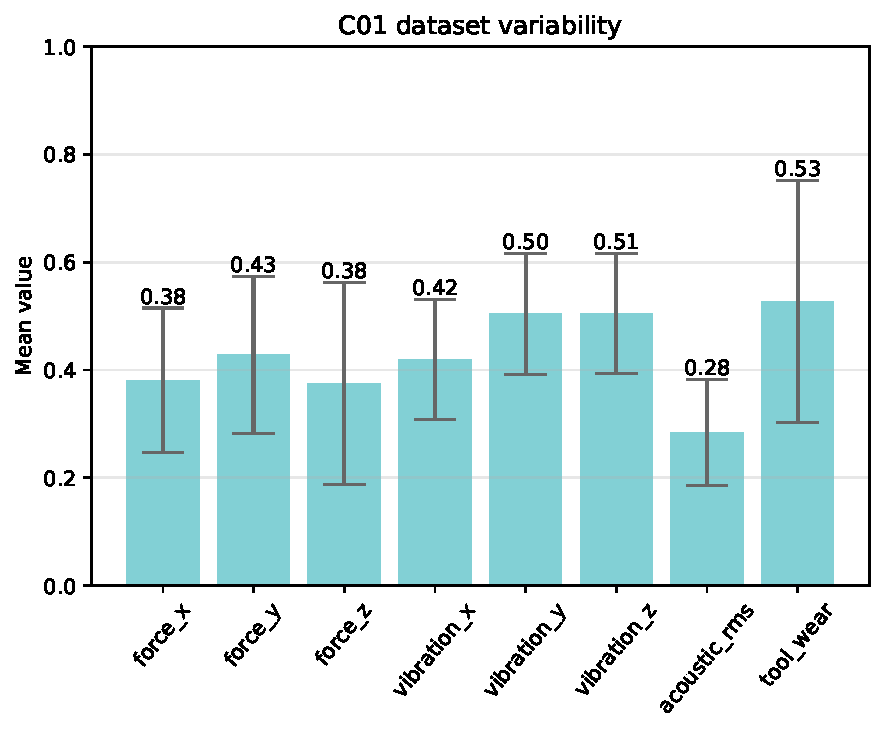
\includegraphics[width=0.325\textwidth]{C01_Features.pdf}}
		\subfigure[\hlc{PHM-C04 dataset}]{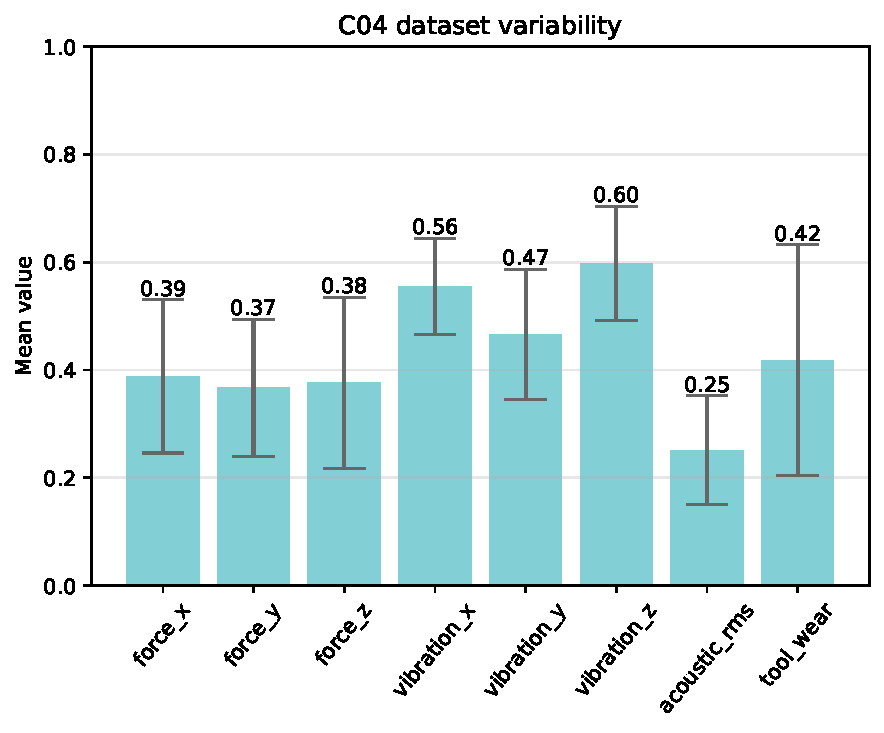
\includegraphics[width=0.325\textwidth]{C04_Features.pdf}}
		\subfigure[\hlc{PHM-C06 dataset}]{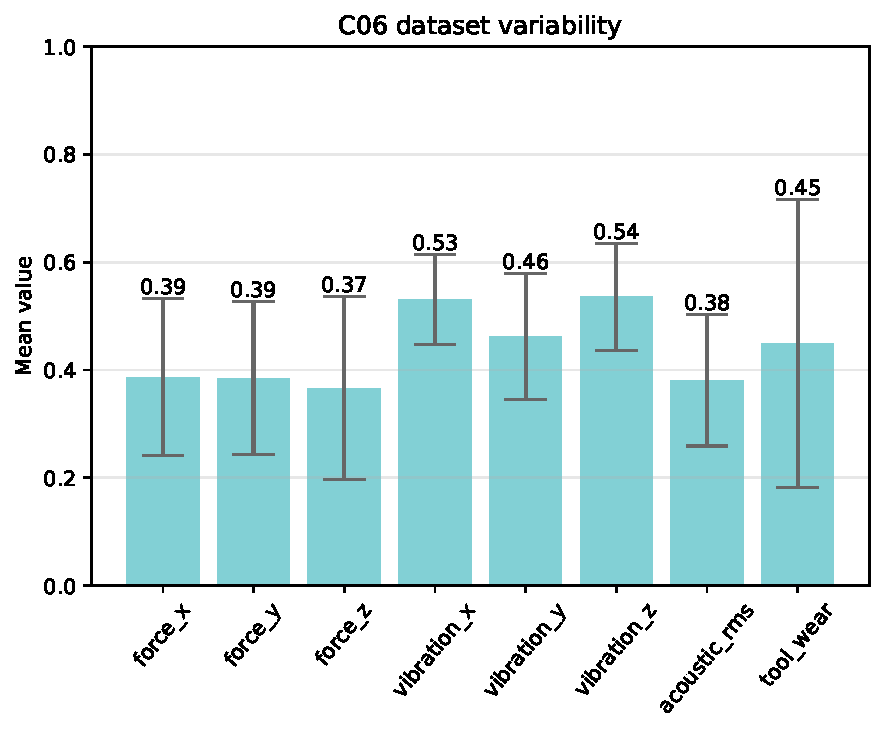
\includegraphics[width=0.325\textwidth]{C06_Features.pdf}}
		\caption{\hlc{Feature variability across datasets. Values are normalized to visualize relative variability.}}
		\label{fig_PHMDataVariability}
	\end{figure}
	\begin{figure}[hbt!]
		\centering
		\includegraphics[width=0.7\textwidth]{PHMMSdata.pdf}  
		\caption{Indicative plot of PHM-C06 multivariate data, showcasing inherent feature complexity. Y-axis indicate magnitude of sensor values. X-axis is number of data-points.}
		\label{fig_PHMMSdata}
	\end{figure} 
	
	
	
	In practice, state variables are often normalized to improve stability and convergence. Both the simulated and real data was normalized using min-max scaling such that the tool wear and other state features, $x \in [0,\;1] \subset \mathbb{R} $. We will see next how this allows adding white noise of similar magnitudes across different PHM datasets.
	
	\subsubsection*{Adding noise and chance of break-down}
	%% $$$ R2-9
	\hlc{Study of noise in RL settings is of prime importance, as suggested by} \cite{Eimer2023AutoRL}. Fig. \ref{fig_noise} shows the effect of adding two levels of noise; a ``low'' level by adding Gaussian noise of order $-3$, $(0.0, 0.001]$ and ``high'' of order $-2$, $(0.0, 0.01]$. Since the tool wear is less than 0.24 mm, this adds significant perturbations as seen in Fig. \ref{fig_LBD} and \ref{fig_HBD}. The noise affects the tool replacement decision (solid blue line) around the replacement threshold (dotted red line). The \textit{human} preventive maintenance policy replaces the tool if the wear exceeds the threshold and this decision boundary oscillates due to the noise. One can see that in the case of no noise (Fig. \ref{fig_NBD}), the decision boundary is clean.
	
	\begin{figure}
		\centering	
		\subfigure[No noise]{\label{fig_NBD}\includegraphics[width=0.65\textwidth]{PHM_C04_NoNBD_wear_plot.png}}
		\subfigure[Low noise]{\label{fig_LBD}\includegraphics[width=0.65\textwidth]{PHM_C04_LowNBD_wear_plot.png}}
		\subfigure[High noise]{\label{fig_HBD}\includegraphics[width=0.65\textwidth]{PHM_C04_HighNBD_wear_plot.png}}
		\caption{PHM C04 tool wear data (normalized) and the effect of noise. Blue line is the replacement action decision.}
		\label{fig_noise}
	\end{figure}
	
	Break down occurs due to excessive tool use and can often occur randomly. In conjunction with Guassian noise this complexity is added for the univariate state based environments. For the low-noise variant we add a low 5\% chance of break down and for the high noise variant we add a higher chance of 10\%. The ``milling'' episode is terminated if a probability, sampled from a uniform distribution is less than this ``chance'' threshold.
	
	Table \ref{tbl_ListEnvironments} summarizes the 15 environment variants and their three logical groups: (1) Simulated 1-3 (2) Real data -- simple univariate environment (4-12) and Real data -- complex multivariate (13-15).
	
	\begin{table}
		\rowspace{1.3}
		\caption{List of the fifteen environments and their categorization.}\label{tbl_ListEnvironments}
		{\begin{tabular}{@{}r l rr@{}} \arrayrulecolor{black!40}\toprule 
				& Environment variant & Noise factor & Breakdown chance \\ \midrule
				& \multicolumn{3}{l}{\textbf{Simulated}}\\
				1 & Simulated - No noise  & None & None \\
				2 & Simulated - Low noise & 1e-3 & 0.05 \\
				3 & Simulated  - High noise & 1e-2 & 0.10 \\ \midrule
				\rule{0pt}{1.5\normalbaselineskip}
				& \multicolumn{3}{l}{\textbf{Real data -- simple univariate}} \\
				4 & PHM C01 SS (simple, univariate) - No noise & None & None \\
				5 & PHM C01 SS (simple, univariate) - Low noise & 1e-3 & 0.05 \\
				6 & PHM C01 SS (simple, univariate) - High noise & 1e-2 & 0.10 \\ \hdashline
				
				7 & PHM C04 SS (simple, univariate) - No noise & None & None \\
				8 & PHM C04 SS (simple, univariate) - Low noise & 1e-3 & 0.05 \\
				9 & PHM C04 SS (simple, univariate) - High noise & 1e-2 & 0.10 \\ \hdashline
				
				10 & PHM C06 SS (simple, univariate) - No noise & None & None \\
				11 & PHM C06 SS (simple, univariate) - Low noise & 1e-3 & 0.05 \\
				12 & PHM C06 SS (simple, univariate - High noise & 1e-2 & 0.10 \\ \midrule
				
				\rule{0pt}{1.5\normalbaselineskip}
				& \multicolumn{3}{l}{\textbf{Real data -- complex multivariate}}\\
				13 & PHM C01 MS (complex, multivariate) - No noise & None & None \\
				14 & PHM C04 MS (complex, multivariate) - No noise & None & None \\
				15 & PHM C06 MS (complex, multivariate) - No noise & None & None \\ \bottomrule
		\end{tabular}}
		
	\end{table}
	
	\subsubsection*{Tool wear as a Markov Decision Processes (MDP)}
	Formulating our problem to be solved by RL requires us to assume that the wear process satisfies the Markov property -- which implies that the transition of tool wear to another state is dependent only on the current state and not on any previous states. MDPs are defined by the tuple $<\mathcal{S, A, P, R, \gamma}>$. We will define the elements of state space $\mathcal{S}$, action space $\mathcal{A}$ and reward function $\mathcal{R}$, next.
	
	\subsubsection*{State and environment elements}
	There are two basic state definitions across the 15 environment variants, the ``simple univariate'' and the ``complex multivariate''. 
	
	The elements of simple univariate state vector are $S_t = [w_t]$, where $w_t$ is the current tool wear. As part of the environment other elements that are sensed by the agent are $[W_\tau, N_f, P_{bd}]$, where $W_\tau$ is the wear threshold, $N_f$ is the noise factor and is one of [0, 1e-3, 1e-2], $P_{bd}$ is the chance of tool breakdown and is one of [0, 0.05, 0.10]. The complex multivariate state $S_t = [f_x, f_y, f_z, v_x, v_y, v_z, ae_{rms}, w_t]$ where, as mentioned in Sec. \ref{sec_PHMdata}, $(f_x, f_y, f_z)$ represents the force along the 3 axes, similarly $v$ represents the vibration, $ae_{rms}$ the acoustic emission.
	
	\subsubsection*{Actions}
	The action space is binary, $\mathcal{A} \in [0, 1]$, where $0$ ($\texttt{CONTINUE}$) represents continuation of milling operation and $1$ ($\texttt{REPLACE\_TOOL}$) represents the action of replacing the tool.
	
	\subsubsection*{Environment feedback}
	``Feedback'' generated by the action an agent takes, is the central mechanism by which agents learn. This is implemented via the \texttt{step()} function in the environment code and is outlined in Algorithm \ref{alg:SSStep}. At every time step an action $A_t$ is taken and the resulting state is evaluated for terminating conditions or assigning a reward and continuing.
	
	\subsubsection*{Reward function}
	\begin{equation}
		R_t \;\;=\;\;
		\begin{cases}
			\;\;  +R_1 \times t, & \quad if \;\; w_t < W_\tau\\
			\;\;  -R_2 \times t, & \quad if \;\; w_t\ge W_\tau\\
			\;\; \mathrel{+}= -R_3, & \quad if \;\; \text{ACTION = REPLACE\_TOOL}\\
		\end{cases}
		\label{eq_RewardFunction}
	\end{equation}
	In the reward function \eqref{eq_RewardFunction} there are three distinct phases where a reward (or penalty) is offered as feedback. $R_1$, $R_2$ and $R_3$ are constants that determine the magnitude of reward. When the current state of wear $w_t$ is less than the threshold $W_\tau$ we have a desirable condition, and we award the agent a positive reward. The formulation {\eqref{eq_RewardFunction}} allows a higher reward to be collected the closer it is to threshold so as to maximize tool usage, but not allowing it to cross it. If it does, the agent is penalized (negative reward) by a magnitude of $R_2$, and once again the farther away it is from the threshold i.e. a highly deteriorated tool the larger the penalty. To avoid this ``bad" state, the agent must learn to replace the tool; represented by the third condition. Tool replacement implies a direct cost (that of the tool) and a much higher and significant downtime ``cost''. To ensure the agent does not learn to replace unnecessarily, we ``penalize'' it. It is important to note that the last condition in {\eqref{eq_RewardFunction}} is an ``incremental addition'', the first two conditions are mutually exclusive and evaluated first, followed by the last condition which is incrementally added on whatever reward is collected in the previous condition. The agent then tries to balance these three conditions, such that it maximizes its total return, over time.
	
	Of the final two elements of the MDP quintuple, $\mathcal{P}$ represents the probability transition matrix and is usually not known and we will therefore use \textit{model-free} RL techniques to learn that from ``experiences''; $\gamma$ enables the agent to learn long-term impact of its actions i.e. what is the long term impact of replacing the tool now or that of delaying the replacement, $\gamma$ is set to 0.99 to facilitate this farsightedness.
	
	\begin{algorithm}[hbt!]
		%	\onehalfspacing
		\caption{Agent class \texttt{step()} method -- Reward handling mechanism}\label{alg:SSStep}
		\begin{algorithmic}[1]
			\Procedure {Step class method: Reward handling}{}\newline
			\textbf{Class attributes:} Wear-threshold $W_\tau$; reward accumulated so far $Reward$; reward function parameters $R1$, $R2$ and $R3$; random chance of breakdown $P_{bd}$; tool replacements made so far $tool\_replacements$; maximum allowable operations $T$\newline
			\textbf{Input:} Current length of episode $t$; current tool-wear $w_t$; current policy action $A_t$;  current index of training data $data\_index$ \newline
			%\textbf{Output:} Predicted tool-wear values $\hat{y}$, computed attention weights $A$\newline
			
			\State \textbf{Initialize} $p$ from uniform probability distribution
			%\LineComment{Termination conditions: Terminate episode, reset reward values and reset\par 
				%				\hskip8pt the training data-frame index to the beginning.}
			%\If {length of episode $\geq$ maximum allowable operations}:
			
			\If {$t \geq T$}:
			\LineComment{Termination based on length of episode.}
			\State $Terminate \gets True$
			\State $Reward \gets 0.0$
			\State $data\_index \gets 0$	\Comment{Reset the training data-frame index to the beginning.}\newline
			
			%\ElsIf {tool-wear is $>$ wear threshold $W_\tau$ AND random-chance of breakdown $P_{bd} >$wear threshold $W_\tau$}
			
			\ElsIf {$w_t > W_\tau$ \textbf{and} $p < P_{bd}$}:
			\LineComment{Termination based on chance of breakdown.}
			
			\State $Terminate \gets True$
			\State $Reward \gets 0.0$
			\State $data\_index \gets 0$		
			\Else
			\State $Terminate \gets False$
			\If {$ w_t < W_\tau $}:
			\LineComment{Healthy tool}
			\State $Reward \gets Reward + t \cdot R1$
			\Else
			\LineComment{Tool deteriorating}
			\State $Reward \gets Reward - t \cdot R2$	
			\EndIf
			\If {$A_t$ is $REPLACE\_TOOL$}:
			\LineComment{Tool is replaced}
			\State $Reward \gets Reward - R3$
			\State $data\_index \gets 0$ \Comment{Tool replaced, therefore roll back tool life}
			\State Increment $tool\_replacements$
			\EndIf			
			\EndIf
			\EndProcedure
		\end{algorithmic}
	\end{algorithm}
	
	\subsubsection*{Network architecture and basic hyperparameters}\label{sec_architecture}
	Stable-Baselines3 (SB3) provides robust open source implementations of many RL algorithms, \cite{SB3-paper}. As of 20-Sep-2024, 13 algorithms have been implemented however REINFORCE has \textit{not} been implemented, \cite{SB3-algorithms}. For this research we use the \textit{default} SB3 implementations of DQN, A2C and PPO and compare its performance to a custom implementation of the REINFORCE algorithm using a very simple network architecture. Table \ref{tbl_network-architecture} shows a comparison of the architecture and the basic common hyperparameters.
	
	\begin{table}
		\rowspace{1.3}
		\caption{Comparing the network architecture and basic hyper-parameters across algorithms.}%\label{tab1}%
		{\begin{tabular}[h]{L{2cm} R{2.5cm} R{2.5cm} R{2.5cm} R{3cm}}
				\arrayrulecolor{black!40}\toprule
				&\textbf{A2C}&\textbf{DQN}&\textbf{PPO}&\textbf{REINFORCE}\\ \midrule
				
				Network\par architecture&input dim x\par [64$\vert$Tanh x 64$\vert$Tanh]\par x output dim&input dim x\par [64$\vert$Tanh x 64$\vert$Tanh]\par x output dim&input dim x\par [64$\vert$Tanh x 64$\vert$Tanh]\par x output dim&input dim x\par [64$\vert$ReLU]\par x output dim\\
				Layers&2&2&2&1\\
				Units&64  x 64&64  x 64&64  x 64&64\\
				Activation&Tanh, Tanh&Tanh, Tanh&Tanh, Tanh&ReLU\\
				Optimizer&RMSprop&Adam&Adam&Adam\\ \midrule
				Learning rate&0.0007&0.0001&0.0003&0.01\\
				Gamma&0.99&0.99&0.99&0.99\\			
				\bottomrule
		\end{tabular}}
		%	\tabnote{\textsuperscript{a}This footnote shows how to include footnotes to a table if required.}
		\label{tbl_network-architecture}
	\end{table}
	
	The REINFORCE uses a \textit{single} internal layer of 64 units. The default architecture for all three SB3 algorithms (A2C/DQN/PPO) consists of \textit{two} fully connected layers with 64 units per layer \cite{SB3-DefaultNetwork}. While REINFORCE used ReLU (rectified linear unit) as the activation function, the other three algorithms used hyperbolic tangent (Tanh). Finally, REINFORCE's learning-rate is much larger.
	
	
	\subsection{Training}
	The training strategy must ensure a uniform comparison of the algorithms. We maintained the exact \textit{same} environment variant, wear dataset, noise parameter, probability of breakdown parameter, and the three reward function parameters; across all four algorithms during a single training round. %Our code is fairly automated and we used a configuration file to configure the training experiments and record the test results. Fig. \ref{fig_exptconfig} shows the main columns of the configuration file we used.
	As the wear data is time-series data, the training and test sets are created by systematic sampling. Simulated data and real tool wear data (PHM) was randomly sampled at a certain frequency and down sampled into training and test sets.
	
	The REINFORCE was trained for 800 episodes for the simulated and PHM univariate variants, for all three noise and breakdown levels (none, low and high) -- Table \ref{tbl_ListEnvironments} items 1-12. For the PHM multivariate variant, Table \ref{tbl_ListEnvironments} items 13-15, REINFORCE was trained for 1000 episodes. SB3 algorithms were trained for 10,000 episodes for all variants. We ran ten rounds of training, tested each generated model and averaged results over the 10 rounds. Testing is explained in the next section while results are presented in Sec. \ref{sec_Results}.
	
	\begin{figure}
		\centering	
		\subfigure[PHM C04 wear data]{\label{fig_C04wear}\includegraphics[width=0.45\textwidth]{7_PHM_C04_SS_LowNBD__wear_plot.png}}
		\subfigure[Average rewards per episode]{\label{fig_C04rewards}\includegraphics[width=0.45\textwidth]{7_PHM_C04_SS_LowNBD__Avg_episode_rewards.png}}
		\hfill
		\subfigure[Episode length completed per episode]{\label{fig_C04eplen}\includegraphics[width=0.45\textwidth]{7_PHM_C04_SS_LowNBD__Episode_Length.png}}		
		\subfigure[Tool replacements per episode]{\label{fig_C04toolrep}\includegraphics[width=0.45\textwidth]{7_PHM_C04_SS_LowNBD__Tool_Replacements.png}}
		\caption{Training plots of REINFORCE. Dataset: PHM-C04. Variant: Univariate state, low-noise and low chance of breakdown.}
		\label{fig_C04trplots}
	\end{figure}
	
	Fig. \ref{fig_C04trplots} shows the training plots for the algorithm of our interest -- REINFORCE. It displays how the wear plot looked for C04 with low noise and low chance of breakdown settings. The average rewards increase over the course of 800 episodes (Fig. \ref{fig_C04rewards}). The episode length (Fig. \ref{fig_C04eplen}) demonstrates the complexity introduced by random breakdown (which abruptly terminates the episode). It is the tool replacement policy that is of interest to the industrial practitioner -- Fig. \ref{fig_C04toolrep} shows that it decreases to optimal levels as the agent learns over time. Similarly, Fig. \ref{fig_C06trplots} demonstrates the training for the PHM C06 dataset affected by high noise and higher breakdown probability. Finally, for the more complex multivariate state variant, the training plots are as seen in Fig. \ref{fig_C01trplots}; as we do not introduce noise or breakdown here, the episodes are always completed (Fig. \ref{fig_C01eplen}).
	
	\begin{figure}
		\centering	
		\subfigure[PHM C06 wear data]{\label{fig_C06wear}\includegraphics[width=0.45\textwidth]{11_PHM_C06_SS_HighNBD__wear_plot.png}}
		\subfigure[Average rewards per episode]{\label{fig_C06rewards}\includegraphics[width=0.45\textwidth]{11_PHM_C06_SS_HighNBD__Avg_episode_rewards.png}}
		\hfill
		\subfigure[Episode length completed per episode]{\label{fig_C06eplen}\includegraphics[width=0.45\textwidth]{11_PHM_C06_SS_HighNBD__Episode_Length.png}}		
		\subfigure[Tool replacements per episode]{\label{fig_C06toolrep}\includegraphics[width=0.45\textwidth]{11_PHM_C06_SS_HighNBD__Tool_Replacements.png}}
		\caption{Training plots of REINFORCE. Dataset: PHM-C06. Variant: Univariate state, high-noise and high chance of breakdown.}
		\label{fig_C06trplots}
	\end{figure}
	
	\begin{figure}
		\centering	
		\subfigure[PHM C01 wear data]{\label{fig_C01wear}\includegraphics[width=0.45\textwidth]{0_0_PHM_C01_MS_NoNBD__wear_plot.png}}
		\subfigure[Average rewards per episode]{\label{fig_C01rewards}\includegraphics[width=0.45\textwidth]{0_0_PHM_C01_MS_NoNBD__Avg_episode_rewards.png}}
		\hfill
		\subfigure[Episode length completed per episode]{\label{fig_C01eplen}\includegraphics[width=0.45\textwidth]{0_0_PHM_C01_MS_NoNBD__Episode_Length.png}}		
		\subfigure[Tool replacements per episode]{\label{fig_C01toolrep}\includegraphics[width=0.45\textwidth]{0_0_PHM_C01_MS_NoNBD__Tool_Replacements.png}}
		\caption{Training plots of REINFORCE. Dataset: PHM-C01. Variant: Multivariate state, No noise or breakdown.}
		\label{fig_C01trplots}
	\end{figure}
	
	\subsection{Testing and performance evaluation}
	Testing was performed with data separate from the training data. 10 rounds of testing are performed, with a \textit{new} set of 40 test cases randomly sampled and frozen across all four algorithms, during each round.
	
	\subsubsection*{Evaluation metrics}
	The human decision is based on ``preventive maintenance'' -- replace the tool against a predefined wear threshold. In our data a tool replacement is represented as 1 and a normal operation as 0. We applied classification metrics to evaluate the RL agent decisions of tool replacement. %These are simple to understand for the general industrial practitioners against other RL evaluation methods such as average reward or the number of episodes to reach maximum reward. 
	It is worth noting that while we have selected an arbitrary wear threshold as this serves our purpose for algorithm comparison; in reality the threshold is based on several factors like materials of tool and work-piece, the duration of continuous operation, ambient conditions, ``cost'' of production downtime etc. Threshold could therefore vary significantly from one case to another. 
	\begin{figure}[hbt!]
		\begin{center}
			\sffamily
			\rowspace{1.6}
			%\begin{tabular}{l|l|c|c|}
			\begin{tabular}{llcc}
				\multicolumn{2}{c}{}&\multicolumn{2}{c}{\textbf{Human decision}}\\
				\cmidrule(lr){3-4}
				%\cline{3-4}
				%\multicolumn{2}{c|}{}&Replace tool&Continue milling\\
				\multicolumn{2}{c}{}&Replace tool&Continue milling\\
				\cmidrule(lr){2-4}
				%\cline{2-4}
				\multirow{2}{*}{\textbf{Agent decision}}& Replace tool & $TP$& $FP$\\
				\cmidrule(lr){2-4}
				%\cline{2-4}
				& Continue milling& $FN$& $TN$\\
				\cmidrule(lr){2-4}
				%\cline{2-4}
			\end{tabular}
		\end{center}
		\caption{Confusion matrix: Human versus Agent decisions}
		\label{fig_CM}	
	\end{figure}
	
	Classification metrics are based on the confusion matrix shown in Fig. \ref{fig_CM}. $TP$ represents true positive cases, where both the agent and human agree on replacing the tool. False positive $FP$ cases denote the agent falsely suggesting replacements, while false negatives $FN$ are cases where continuation of milling is suggested, when in fact a tool replacement would have helped. Precision (Pr), Recall (Rc) and F1-score metrics can then be computed as shown in \eqref{eq_metrics}.
	
	\begin{equation}
		\text{Pr} = \frac{TP}{TP+FP}, \quad
		\text{Rc} = \frac{TP}{TP+FN}, \quad
		\text{F1-score} = 2 \times \frac{Pr \times Rc)}{(Pr + Rc)}
		\label{eq_metrics}
	\end{equation}
	
	%% $$$ R1-3
	\hlc{For a classification problem, the choice of precision versus recall will depend on the industry and application}. Timely replacements, $TP$, ensure work piece quality \hlc{while still maintaining minimal production downtime. Precision is driven by lower $FP$s i.e. reducing unnecessary replacements. A high recall is necessary in several critical industrial environments, where failing to replace the tool can lead to serious consequences, demanding lower $FN$s.} \hlc{Depending on the industrial application one can use a \textit{weighted} F1-score equation} (\ref{eq_Fbeta}) \hlc{that is oriented toward precision or recall}. For high precision applications set a $\beta < 1.0$; \hlc{for applications demanding higher recall, set a $\beta > 1.0$.} For \hlc{this research} we set $\beta$ to $0.5$ and \hlc{suggest setting $\beta$ to $2.0$ for applications where recall is critical}.
	
	\begin{equation}
		F_{\beta} = (1+\beta^2) \cdot \frac{(Pr \times Rc)}{(\beta^2 \cdot Pr + Rc)}
		\label{eq_Fbeta}
	\end{equation}
	
	%% $$$ R1-6	CI
	\hlc{Throughout the article we use 95\% confidence intervals (CI) to quantify the uncertainty of the metrics and provide an indication of the robustness. In the Results Sec. {\ref{sec_Results}}, these are presented in the results tables (columns titled '95\% CI') and as error-bars in the accompanying plots.}
	
	\section{Results}\label{sec_Results}
	We present the summarized results in this section accompanied by commentary referring to detailed results made available in Appendix \ref{apx}. Since there are several tables and figures, for reference, we created a cross-linked Table \ref{tbl_ref-results}. Generally, \textcolor{dblue}{blue} text is used in tables to highlight prominent values. Summary performance and F$_\beta$0.5 plots accompany tables to assist in visualizing the comparative performance. The F$_\beta$0.5 plots show \textit{individual} performance over ten rounds of training-validation and help infer training stability. Similar plots for precision, recall and F1 have been relegated to Appendix \ref{apx}.
	
	\begin{table}
		\rowspace{1.3}
		\caption{Reference table for results.}
		{\begin{tabular}{R{0.25cm} L{11.5cm} L{3cm}}
				\arrayrulecolor{black!40}\toprule 
				& Item & Reference\\ \midrule
				\rowcolor{ltgray} & \textbf{Summary Results}  & \\ 
				
				1 & Overall summary -- All 15 environments, averaged over 10 rounds & Table \ref{tbl_OverallSummary}, Fig. \ref{fig_OverallSummary}\\
				& \quad\quad --"-- \quad F$_\beta$0.5 behavior plot over 10 rounds & Fig. \ref{fig_FbetaOverall}\\\ltmidrule
				
				2 & Simple univariate state -- Simulated data, 3 variants (3 noise settings), averaged over 10 rounds & Table \ref{tbl_SimulatedEnv}, Fig. \ref{fig_SimulatedEnv}\\ 
				& \quad\quad --"-- \quad F$_\beta$0.5 behavior plot over 10 rounds & Fig. \ref{fig_FbetaSimulated}\\\ltmidrule
				
				3 & Simple univariate state -- Real data, 9 variants (3 datasets $\times$ 3 noise settings), averaged over 10 rounds & Table \ref{tbl_PHMSS}, Fig. \ref{fig_PHMSS}\\
				& \quad\quad --"-- \quad F$_\beta$0.5 behavior plot over 10 rounds & Fig. \ref{fig_FbetaPHMSS}\\\ltmidrule
				
				4 & Complex multivariate state -- Real data, 3 variants (3 datasets), averaged over 10 rounds & Table \ref{tbl_PHMMS}, Fig. \ref{fig_PHMMS}\\
				& \quad\quad --"-- \quad F$_\beta$0.5 behavior plot over 10 rounds & Fig. \ref{fig_FbetaPHMMS}\\\ltmidrule
				
				\rowcolor{ltgray} & \textbf{Super Models}  & \\ 
				5 & Super Models -- Best model, \textit{averaged} over all 15 environments & Table \ref{tbl_supermodels} Fig. \ref{fig_supermodels}\\
				& Super Models -- Best model, \textit{details} of all 15 environments & Appendix \ref{apx} - Table \ref{tbl_SuperModelsDetailedMetrics}\\\ltmidrule
				
				\rowcolor{ltgray} & \textbf{Hypothesis tests and Training time results}  & \\ 
				6 & Hypothesis tests -- p-value and t-statistic of REINFORCE versus other algorithms & Table \ref{tbl_ttest}\\
				7 & Training time -- Averaged over 10 rounds and all 15 variants & Fig. \ref{fig_tr-time}\\\ltmidrule
				
				\rowcolor{ltgray} & \textbf{Detailed Results} - Appendix \ref{apx} & \\
				8 & Complete detailed results -- All 15 environments, averaged over 10 rounds & Appendix \ref{apx} - Table \ref{tbl_DetailedMetrics}\\\ltmidrule
				
				9 & Stability behavior plots over 10 rounds, Precision, Recall and F1\\
				& \quad\quad Overall (all variants)  & Appendix \ref{apx} - Fig. \ref{fig_tr-overall}\\
				& \quad\quad Simulated state & Appendix \ref{apx} - Fig. \ref{fig_tr-sim-env}\\
				& \quad\quad Simple univariate state & Appendix \ref{apx} - Fig. \ref{fig_tr-ss-env}\\
				& \quad\quad Complex multivariate state & Appendix \ref{apx} - Fig. \ref{fig_tr-ms-env}\\
				\bottomrule
		\end{tabular}}
		\label{tbl_ref-results}
	\end{table}
	
	\subsection{Overall performance}
	% $$$: CI R1-6	
	\begin{table}
		\rowspace{1.3}
		\caption{\hlc{Model performance summary - averaged over all environments.}}
		{\begin{tabular}
				{@{}l rrr c rrr c rrr c rrr@{}}
				\arrayrulecolor{black!40}\toprule
				& \multicolumn{3}{c}{Precision} &  & \multicolumn{3}{c}{Recall} & & \multicolumn{3}{c}{F1-score} &  & \multicolumn{3}{c}{F$_\beta$0.5} \\
				\cmidrule{2-4} \cmidrule{6-8} \cmidrule{10-12} \cmidrule{14-16} 
				&Mean &SD &\hlc{95\% CI} & &Mean &SD &\hlc{95\% CI} & &Mean &SD &\hlc{95\% CI} & &Mean & SD &\hlc{95\% CI}\\ \midrule						
				A2C & 0.449 & 0.088 & \makecell{(0.443,\\ 0.455)} & &0.480 & 0.084 & \makecell{(0.474,\\ 0.485)} & & 0.442 & 0.070 & \makecell{(0.437,\\ 0.446)} & &0.436 &0.071 & \makecell{(0.431,\\ 0.440)} \\ \arrayrulecolor{gray!30} \midrule
				DQN & 0.418 & 0.185 & \makecell{(0.406,\\ 0.430)} & &0.504 & 0.032 & \makecell{(0.502,\\ 0.506)} & & 0.374 & 0.035 & \makecell{(0.372,\\ 0.376)} & &0.348 &0.058 & \makecell{(0.344,\\ 0.351)} \\\midrule
				PPO & 0.472 & 0.144 & \makecell{(0.463,\\ 0.482)} & &0.316 & 0.087 & \makecell{(0.310,\\ 0.321)} & & 0.345 & 0.091 & \makecell{(0.339,\\ 0.351)} & &0.393 &0.105 & \makecell{(0.386,\\ 0.400)} \\\midrule
				REINFORCE & \textcolor{dblue}{0.687} & 0.059 & \makecell{(0.683,\\ 0.691)} & &\textcolor{dblue}{0.629} & 0.051 & \makecell{(0.626,\\ 0.633)} & & \textcolor{dblue}{0.609} & 0.050 & \makecell{(0.606,\\ 0.612)} & & \textcolor{dblue}{0.631} &0.052 & \makecell{(0.627,\\ 0.634)} \\						
				\bottomrule
		\end{tabular}}
		\label{tbl_OverallSummary}
	\end{table}		
	
	\begin{figure}[hbt!]
		\centering
		\includegraphics[width=0.6\textwidth, trim={1.5cm 7cm 1cm 7cm}]{OverallPlot.pdf}  
		\caption{Overall model performance summary}
		\label{fig_OverallSummary}
	\end{figure}
	At an aggregated level, Table {\ref{tbl_OverallSummary}} along with Fig. {\ref{fig_OverallSummary}}, show that the REINFORCE scores better than the other algorithms, on all four metrics. Tool replacement precision at 0.687, is highest of the four algorithms and better by 0.215 in absolute terms when compared to the next best, PPO. The standard deviation for precision is the lowest at 0.059. On recall, F1 and F$_\beta$0.5, REINFORCE is better by 0.125, 0.168 and 0.195 compared to the next best.
	
	These metrics were averaged over 10 rounds of training followed by validation. We visualize the behavior of our primary metric F$_\beta$0.5, \textit{individually} across the ten rounds in Fig. {\ref{fig_FbetaOverall}}. The blue line floating above the rest of the algorithms, for all metrics, is that of REINFORCE and appears fairly stable across the ten rounds. The error-bars are also pretty small, indicating lower uncertainty. We notice that the other three algorithms are all centered closely around, 0.4.
	\begin{figure}[hbt!]
		\centering
		\includegraphics[width=0.9\textwidth]{Overall_F05.pdf}  
		\caption{Overall performance comparison of the F$_\beta$0.5 metric, over 10 rounds of training and testing.}
		\label{fig_FbetaOverall}
	\end{figure}
	
	We now dig into the detailed metrics Appendix {\ref{apx}} - Table {\ref{tbl_DetailedMetrics}} to better understand the aggregated summary. The largest values are typeset in {\textcolor{dblue}{blue}}. And a quick visual glance shows the dominance of REINFORCE. The notable exceptions are the PHM C01 single-state and no-noise variant where A2C and DQN do better, followed by PHM C01 and PHM C06 univariate-state, low-noise variants where A2C performs better in every aspect and finally the PHM C04 and C06 multivariate variants where A2C again performs better on recall and which in turns drives the F1 score up. Barring these three complete cases and two cases where A2C recall was better, the REINFORCE performs best in ten variants and in two cases its precision, and therefore F$_\beta$0.5, is highest. This corroborates the overall performance observed in Table {\ref{tbl_OverallSummary}}. \hlc{As seen in Table {\ref{tbl_DetailedMetrics}} there are significant variations in performance across the datasets - for \textit{all} algorithms. One reason for this is by design -- the sample datasets we selected had noticeable variation between them, as we saw in Fig. {\ref{fig_PHMDataVariability}}}. Finally, Fig. {\ref{fig_tr-overall}} shows that the stability across multiple rounds is evident for other metrics as well.
	
	\subsection{Simulated environment}
	\begin{table} % $$$: CI R1-6
		\rowspace{1.3}
		\caption{\hlc{Simulated environments - model performance summary.}}
		{\begin{tabular}
				{@{}l rrr c rrr c rrr c rrr@{}}
				\arrayrulecolor{black!40}\toprule
				& \multicolumn{3}{c}{Precision} &  & \multicolumn{3}{c}{Recall} & & \multicolumn{3}{c}{F1-score} &  & \multicolumn{3}{c}{F$_\beta$0.5} \\
				\cmidrule{2-4} \cmidrule{6-8} \cmidrule{10-12} \cmidrule{14-16} 
				&Mean &SD &\hlc{95\% CI} & &Mean &SD &\hlc{95\% CI} & &Mean &SD &\hlc{95\% CI} & &Mean & SD &\hlc{95\% CI}\\ \midrule						
				A2C & 0.416 & 0.120 & \makecell{(0.408,\\ 0.423)} & &0.385 & 0.073 & \makecell{(0.380,\\ 0.390)} & & 0.363 & 0.072 & \makecell{(0.358,\\ 0.367)} & &0.373 &0.082 & \makecell{(0.368,\\ 0.379)} \\
				DQN & 0.432 & 0.184 & \makecell{(0.420,\\ 0.443)} & &0.510 & 0.031 & \makecell{(0.508,\\ 0.512)} & & 0.374 & 0.034 & \makecell{(0.372,\\ 0.376)} & &0.351 &0.056 & \makecell{(0.347,\\ 0.354)} \\
				PPO & 0.500 & 0.178 & \makecell{(0.488,\\ 0.511)} & &0.215 & 0.081 & \makecell{(0.209,\\ 0.220)} & & 0.285 & 0.099 & \makecell{(0.278,\\ 0.291)} & &0.370 &0.122 & \makecell{(0.362,\\ 0.378)} \\
				REINFORCE & \textcolor{dblue}{0.806} & 0.040 & \makecell{(0.803,\\ 0.808)} & &\textcolor{dblue}{0.915} & 0.038 & \makecell{(0.913,\\ 0.918)} & & \textcolor{dblue}{0.841} & 0.035 & \makecell{(0.839,\\ 0.844)} & &\textcolor{dblue}{0.816} &0.037 & \makecell{(0.813,\\ 0.818)} \\		
				\bottomrule
		\end{tabular}}
		\label{tbl_SimulatedEnv}
	\end{table}		
	
	\begin{figure}[hbt!]
		\centering
		\includegraphics[width=0.6\textwidth, trim={1.5cm 7cm 1cm 7cm}]{SimulatedPlot.pdf}  
		\caption{Simulated environments - model performance summary.}
		\label{fig_SimulatedEnv}
	\end{figure}
	The simulated tool-wear environment is relatively the simplest for the agent to learn, even with added noise and chance of breakdown. Table \ref{tbl_SimulatedEnv} shows the averaged performance over the three variants. The REINFORCE performs the best and in absolute terms it is better than the next best advanced algorithm by very high margins: precision by 0.306, recall by 0.405, F1 by 0.468 and F$_\beta$0.5 by 0.442, with standard deviation lower or marginally higher than others. F$_\beta$0.5 plot Fig. \ref{fig_FbetaSimulated} shows an exceptionally consistent performance, over all ten trained models, vis-a-vis the other algorithms. Plot Fig. \ref{fig_tr-sim-env} shows DQN fluctuating heavily, occasionally showing recalls at the REINFORCE levels (rounds 2 and 8).
	\begin{figure}[hbt!]
		\centering
		\includegraphics[width=0.9\textwidth]{Simulated_F05.pdf}  
		\caption{Simulated environments - F$_\beta$0.5 metric, over 10 rounds of training and testing.}
		\label{fig_FbetaSimulated}
	\end{figure}
	
	\subsection{Real data - simple univariate environment}
	\begin{table} % $$$: CI R1-6
		\rowspace{1.3}
		\caption{\hlc{Model performance summary - averaged over PHM-2010 environments with simple single-variable environment.}}
		{\begin{tabular}
				{@{}l rrr c rrr c rrr c rrr@{}}
				\arrayrulecolor{black!40}\toprule
				& \multicolumn{3}{c}{Precision} &  & \multicolumn{3}{c}{Recall} & & \multicolumn{3}{c}{F1-score} &  & \multicolumn{3}{c}{F$_\beta$0.5} \\
				\cmidrule{2-4} \cmidrule{6-8} \cmidrule{10-12} \cmidrule{14-16} 
				&Mean &SD &\hlc{95\% CI} & &Mean &SD &\hlc{95\% CI} & &Mean &SD &\hlc{95\% CI} & &Mean & SD &\hlc{95\% CI}\\ \midrule						
				A2C & 0.447 & 0.077 & \makecell{(0.442,\\ 0.452)} & &0.477 & 0.091 & \makecell{(0.471,\\ 0.483)} & & 0.452 & 0.072 & \makecell{(0.448,\\ 0.457)} & &0.446 &0.070 & \makecell{(0.442,\\ 0.451)} \\
				DQN & 0.419 & 0.179 & \makecell{(0.408,\\ 0.431)} & &0.507 & 0.032 & \makecell{(0.505,\\ 0.509)} & & 0.379 & 0.036 & \makecell{(0.376,\\ 0.381)} & &0.352 &0.057 & \makecell{(0.348,\\ 0.355)} \\
				PPO & 0.450 & 0.146 & \makecell{(0.440,\\ 0.459)} & &0.314 & 0.082 & \makecell{(0.309,\\ 0.319)} & & 0.333 & 0.087 & \makecell{(0.327,\\ 0.339)} & &0.374 &0.102 & \makecell{(0.367,\\ 0.381)} \\
				REINFORCE & \textcolor{dblue}{0.605} & 0.046 & \makecell{(0.602,\\ 0.608)} & &\textcolor{dblue}{0.603} & 0.046 & \makecell{(0.600,\\ 0.606)} & & \textcolor{dblue}{0.570} & 0.041 & \makecell{(0.567,\\ 0.572)} & &\textcolor{dblue}{0.576} &0.040 & \makecell{(0.574,\\ 0.579)} \\		
				\bottomrule
		\end{tabular}}
		\label{tbl_PHMSS}
	\end{table}		
	
	\begin{figure}[hbt!]
		\centering
		\includegraphics[width=0.6\textwidth, trim={1.5cm 7cm 1cm 7cm}]{PHMSSPlot.pdf}  
		\caption{PHM real data - Model performance summary for the simple single-variable environment.}
		\label{fig_PHMSS}
	\end{figure}
	Real data offers a more challenging environment. Despite this, in Table \ref{tbl_PHMSS}, we notice that REINFORCE still performs better than the other algorithms. The margins are understandably lower: precision by 0.155, recall by 0.097, F1 by 0.117 and F$_\beta$0.5 by 0.130. For these variants the F$_\beta$0.5 plot Fig. \ref{fig_FbetaSimulated} shows a considerably higher performance over 9 of the 10 training rounds. Behavior of the other metrics is seen in Fig. \ref{fig_tr-ss-env}. While the REINFORCE precision is higher for most rounds, the recall seems to be occasionally surpassed slightly by DQN's (rounds 1, 8 and 9) and by a larger margin once (round 5).
	\begin{figure}[hbt!]
		\centering
		\includegraphics[width=0.9\textwidth]{Singevariable_F05.pdf}  
		\caption{Univariate simple state environments - F$_\beta$0.5 metric, over 10 rounds of training and testing.}
		\label{fig_FbetaPHMSS}
	\end{figure}
	
	\subsection{Real data - complex multivariate state}
	\begin{table} % $$$: CI R1-6
		\rowspace{1.3}
		\caption{\hlc{Model performance summary - averaged over PHM-2010 environments with complex multivariate environment.}}
		{\begin{tabular}
				{@{}l rrr c rrr c rrr c rrr@{}}
				\arrayrulecolor{black!40}\toprule
				& \multicolumn{3}{c}{Precision} &  & \multicolumn{3}{c}{Recall} & & \multicolumn{3}{c}{F1-score} &  & \multicolumn{3}{c}{F$_\beta$0.5} \\
				\cmidrule{2-4} \cmidrule{6-8} \cmidrule{10-12} \cmidrule{14-16} 
				&Mean &SD &\hlc{95\% CI} & &Mean &SD &\hlc{95\% CI} & &Mean &SD &\hlc{95\% CI} & &Mean & SD &\hlc{95\% CI}\\ \midrule						
				A2C & 0.487 & 0.086 & \makecell{(0.481,\\ 0.492)} & &\textcolor{dblue}{0.582} & 0.075 & \makecell{(0.577,\\ 0.587)} & & 0.488 & 0.063 & \makecell{(0.484,\\ 0.493)} & &0.467 &0.065 & \makecell{(0.463,\\ 0.472)} \\
				DQN & 0.399 & 0.204 & \makecell{(0.386,\\ 0.412)} & &0.491 & 0.032 & \makecell{(0.489,\\ 0.493)} & & 0.361 & 0.035 & \makecell{(0.358,\\ 0.363)} & &0.332 &0.060 & \makecell{(0.328,\\ 0.336)} \\
				PPO & 0.512 & 0.107 & \makecell{(0.505,\\ 0.518)} & &0.422 & 0.107 & \makecell{(0.414,\\ 0.429)} & & 0.441 & 0.096 & \makecell{(0.435,\\ 0.447)} & &0.472 &0.096 & \makecell{(0.465,\\ 0.478)} \\
				REINFORCE & \textcolor{dblue}{0.813} & 0.119 & \makecell{(0.805,\\ 0.821)} & &0.421 & 0.079 & \makecell{(0.416,\\ 0.426)} & &\textcolor{dblue}{0.495} & 0.090 & \makecell{(0.489,\\ 0.501)} & &\textcolor{dblue}{0.609} &0.101 & \makecell{(0.602,\\ 0.615)} \\
				\bottomrule
		\end{tabular}}
		\label{tbl_PHMMS}
	\end{table}
	\begin{figure}[hbt!]
		\centering
		\includegraphics[width=0.6\textwidth, trim={1.5cm 7cm 1cm 7cm}]{PHMMSPlot.pdf}  
		\caption{PHM real data - Model performance summary for the complex multivariate environment.}
		\label{fig_PHMMS}
	\end{figure}
	This environment offers the highest difficulty. We use real data, from \textit{multiple} sensors. As with other scenarios, we used untuned, default settings of all algorithms. In Table \ref{tbl_PHMSS}, we see that the REINFORCE has the poorest recall at 0.421, however it demonstrates a surprisingly high tool replacement precision at 0.813, which drives the F1 and F$_\beta$0.5 to the top of the table. F$_\beta$0.5 performance is reflected in the Fig. \ref{fig_FbetaSimulated}; where it remains high for most rounds. The plot, in Appendix \ref{apx}, Fig. \ref{fig_tr-ms-env} shows REINFORCE's high precision behavior. However, it is important to note that the error-bars are occasionally larger (rounds 0, 2, 4 and 6). The recall seemed higher at some points but lower half the times and this manifests in the F1 behavior.
	\begin{figure}[hbt!]
		\centering
		\includegraphics[width=0.9\textwidth]{Multivariate_F05.pdf}  
		\caption{Multivariate complex state environments - F$_\beta$0.5 metric, over 10 rounds of training and testing.}
		\label{fig_FbetaPHMMS}
	\end{figure}
	
	\subsection{Super models}
	Finally, we look at performance of ``select'' models. Logically, one would choose the best model from a set of 10 trained models, just as an AutoML or AutoRL framework would. Selecting models based on the highest F1 with a \textit{minimum} satisfying criteria for precision and recall allowed us to evaluate performance of ``super-models'' for each algorithm. At an overall averaged level Table \ref{tbl_supermodels} demonstrates the remarkable performance of the simple REINFORCE algorithm. It does show a lower recall when compared to the DQN, however it is a much more \textit{balanced} model on an overall basis. Appendix \ref{apx} Table \ref{tbl_SuperModelsDetailedMetrics} shows details where the REINFORCE performs better than the other three algorithms by a huge margin, for 14 of the 15 variants. For PHM C06, univariate environment, it was the DQN that performed best, with extremely high metrics throughout and an F1 of 0.969 to 0.831 of REINFORCE.
	
	\begin{table} % $$$: CI R1-6
		\rowspace{1.3}
		\caption{\hlc{Super models: Best of 10 rounds; performance averaged over all 15 environments.}}
		{\begin{tabular}
				{@{}l rrr c rrr c rrr c rrr@{}}
				\arrayrulecolor{black!40}\toprule
				& \multicolumn{3}{c}{Precision} &  & \multicolumn{3}{c}{Recall} & & \multicolumn{3}{c}{F1-score} &  & \multicolumn{3}{c}{F$_\beta$0.5} \\
				\cmidrule{2-4} \cmidrule{6-8} \cmidrule{10-12} \cmidrule{14-16} 
				&Mean &SD &\hlc{95\% CI} & &Mean &SD &\hlc{95\% CI} & &Mean &SD &\hlc{95\% CI} & &Mean & SD &\hlc{95\% CI}\\ \midrule	
				
				A2C & 0.520 & 0.031 & \makecell{(0.518,\\ 0.522)} & &0.859 & 0.053 & \makecell{(0.855,\\ 0.862)} & & 0.639 & 0.036 & \makecell{(0.636,\\ 0.641)} & &0.560 &0.032 & \makecell{(0.558,\\ 0.563)} \\
				DQN & 0.651 & 0.022 & \makecell{(0.649,\\ 0.652)} & &0.937 & 0.031 & \makecell{(0.935,\\ 0.939)} & & 0.740 & 0.022 & \makecell{(0.739,\\ 0.742)} & &0.678 &0.021 & \makecell{(0.677,\\ 0.680)} \\
				PPO & 0.558 & 0.076 & \makecell{(0.553,\\ 0.563)} & &0.643 & 0.097 & \makecell{(0.636,\\ 0.649)} & & 0.580 & 0.079 & \makecell{(0.575,\\ 0.585)} & &0.562 &0.075 & \makecell{(0.557,\\ 0.567)} \\
				REINFORCE & \textcolor{dblue}{0.884} & 0.042 & \makecell{(0.881,\\ 0.887)} & &\textcolor{dblue}{0.884} & 0.042 & \makecell{(0.882,\\ 0.887)} & & \textcolor{dblue}{0.873} & 0.034 & \makecell{(0.871,\\ 0.875)} & &\textcolor{dblue}{0.876} &0.036 & \makecell{(0.873,\\ 0.878)} \\				
				\bottomrule
		\end{tabular}}
		\label{tbl_supermodels}
	\end{table}
	
	\begin{figure}[htb]
		\centering
		\includegraphics[width=0.6\textwidth, trim={1.5cm 7cm 1cm 7cm}]{SuperModelsPlot.pdf}  
		\caption{Super models: Best of 10 rounds; performance averaged over all 15 environments.}
		\label{fig_supermodels}
	\end{figure}
	
	\subsection{Hypothesis testing}\label{sec_Hypothesistesting}
	We undertake a statistical analysis of the results, postulated by the hypothesis (\ref{eq_Hypothesis}), \hlc{where the subscripts \textit{RF} and \textit{AA} stand for REINFORCE and ``advanced algorithms'' respectively.} Table \ref{tbl_ttest} shows the result of a one-sided, two-sample t-test, conducted for a significance level $\alpha=0.05$. Sample size of the test are mentioned against each category\footnote{What does a single data point indicate?: Consider the ``Simulated'' category -- 10 training rounds $\times$ 10 test rounds $\times$ 3 noise settings = 300 sample points. Note that a single test round is conducted with 40 randomly sampled wear datapoints and therefore 300 samples = 300 $\times$40 i.e. 12,000 samples of wear data. Similarly, for the real-data univariate state: 3 datasets $\times$ 10 training rounds $\times$ 10 test rounds $\times$3 noise settings = 900 sample points.}.
	\begin{equation}
		\left.\begin{aligned}
			H_0 & : \mu_{RF} - \mu_{AA} = 0,\;\; \\
			H_a & : \mu_{RF} - \mu_{AA} > 0, \;\;
		\end{aligned}
		\right\}
		\qquad \forall \;\; \text{$AA \in[A2C, DQN, PPO]$}
		\label{eq_Hypothesis}
	\end{equation}
	We see that the p-values are extremely low and test statistic positive, for all cases except for the \textit{recall} in the PHM multivariate state case. We can thus reject $H_0$.
	\begin{table}
		\rowspace{1.3}
		\caption{Statistical test: One-sided two-sample t-tests. $H_0: \mu_{RF}-\mu_{AA}=0; H_a: \mu_{RF}-\mu_{AA} > 0$, where $AA$ is one of A2C, DQN or PPO.}
		{\begin{tabular}{@{}l c rrr c l rrr @{}}
				\arrayrulecolor{black!40}\toprule
				
				&& \multicolumn{3}{c}{\textbf{p Value}} & \phantom{i} & & \multicolumn{3}{c}{\textbf{t Statistic}} \\
				\cmidrule{3-5} \cmidrule{8-10} 
				
				Metric && \small {RF $\underset{H_0}{\overset{H_a}{\geqq}}$A2C} &\small {RF $\underset{H_0}{\overset{H_a}{\geqq}}$DQN} &\small {RF $\underset{H_0}{\overset{H_a}{\geqq}}$PPO} & & & \small {RF $\underset{H_0}{\overset{H_a}{\geqq}}$A2C} &\small {RF $\underset{H_0}{\overset{H_a}{\geqq}}$DQN} &\small {RF $\underset{H_0}{\overset{H_a}{\geqq}}$PPO} \\ \midrule 
				\multicolumn{10}{@{}l}{\textbf{Overall} (1500 samples)} \\[6pt]
				Precision & &4.31E-126 &2.17E-109 &2.81E-106 & & &25.071 &23.170 &22.804\\
				Recall & &4.20E-35 &3.37E-16 &4.36E-150 & & &12.522 &8.206 &27.650\\
				F1 score & &1.99E-64 &1.46E-88 &5.29E-155 & & &17.364 &20.634 &28.160\\[6pt]\midrule
				
				\multicolumn{10}{@{}l}{\textbf{Simulated environment} (300 samples)}\\[6pt]
				Precision & &3.20E-98 &1.69E-63 &2.65E-81 & & &25.611 &19.032 &22.427\\
				Recall & &8.12E-104 &2.56E-41 &1.57E-264 & & &26.665 &14.558 &62.541\\
				F1 score & &9.60E-134 &8.56E-99 &2.96E-242 & & &32.402 &25.719 &56.575\\[6pt] \midrule
				
				\multicolumn{10}{@{}l}{\textbf{PHM Real data - Simple univariate state} (900 samples)} \\[6pt]
				Precision & &2.27E-32 &7.29E-31 &9.95E-31 & & &12.082 &11.770 &11.742\\
				Recall & &1.27E-16 &1.55E-06 &8.19E-71 & & &8.357 &4.821 &18.607\\
				F1 score & &1.94E-19 &4.67E-34 &2.19E-67 & & &9.121 &12.423 &18.098\\ [6pt]\midrule
				
				\multicolumn{10}{@{}l}{\textbf{PHM Real data - Complex multivariate state} (300 samples)}\\[6pt]
				Precision & &1.64E-60 &3.34E-54 &7.88E-59 & & &18.451 &17.207 &18.122\\
				Recall & &2.69E-10 &2.69E-02 &9.68E-01 & & &-6.425 &-2.219 &-0.041\\
				F1 score & &7.27E-01 &1.44E-08 &1.35E-03 & & &0.349 &5.748 &3.220\\
				\bottomrule
		\end{tabular}}
		\label{tbl_ttest}
	\end{table}
	
	\subsubsection{Training times \hlc{and model byte size}}
	Our final set of results are related to the training time required \hlc{and size of models produced}, for each algorithm. The na\"ive REINFORCE algorithm is extremely slow, with a very high variance in training time, as seen in Fig. \ref{fig_tr-time}.
	\begin{figure}[hbt!]
		\centering
		\includegraphics[width=0.5\linewidth]{Model_training_time.pdf}  
		\caption{Training time, averaged over 10 rounds and all 15 variants.}
		\label{fig_tr-time}
	\end{figure}
	
	%% $$$ R2-2 Runtime
	\hlc{The model sizes produced by all algorithms is extremely small: A2C 89.8 KB, DQN 56.4 KB, PPO 135.5 KB and REINFORCE 121.5 KB. We see that the DQN produced the smallest while the PPO produced the largest.}
	
	%% $$$ Sensitivity analysis
	\subsection{\hlc{Sensitivity analysis of hyperparameters on the REINFORCE algorithm}}\label{sec_SA}		
	\subsubsection*{\hlc{Selection of hyperparameters for analysis}}
	\hlc{RL algorithms are known to be extremely sensitive to hyperparameter and network architecture settings,} \cite{henderson2018deep, andrychowicz2021matters}. \hlc{We conduct a basic hyperparameter interaction and sensitivity analysis in this section. To select the best hyperparameters to conduct the sensitivity analysis, we referred to recent research} \cite{autorl:shala2022}, \cite{Eimer2023AutoRL},  \hlc{and} \cite{Lavet2016}. \cite{autorl:shala2022} \hlc{created the ``AutoRL-Bench 1.0'' for benchmarking AutoRL performance. We selected the {\textit{same}} common hyperparameters they studied across all RL algorithms they benchmark i.e. learning rate and the discount factor $\gamma$.} \cite{Lavet2016} \hlc{studied empirically, the impact of exactly these two hyperparameters and their impact on performance and instabilities of RL neural networks. Finally, } \cite{Eimer2023AutoRL} \hlc{mention how some often overlooked hyperparameters, such as the discount factor, significantly impacts the algorithm's performance. In addition to these suggestions, we selected the network activation function for analysis, thus covering network architecture as well.}
	
	\hlc{\textbf{Our hyperparameter space}:} \vspace{-6pt}
	\begin{enumerate}    
		\item \hlc{Learning rate: $1\times10^{-4}$, $5\times10^{-4}$, $1\times10^{-3}$, $ 5\times10^{-3}$, $1\times10^{-2}$}
		\item \hlc{Discount factor $\gamma$: $0.90$, $0.95$, $0.99$}
		\item \hlc{Network activation: Hyperbolic Tangent (Tanh) and Rectified Linear Unit (ReLU)}
	\end{enumerate}
	
	\hlc{For our analysis we will train the model and compute the average episodic rewards, over 10 rounds of training. Fig. {\ref{fig_SA_LR_Relu}} shows the impact of changing learning rates on the average episodic rewards, for a particular $\gamma$ value, with the network activation function set to ReLU. Uncertainty is indicated by the light blue region bounded by 95\% CI (confidence intervals). Similarly Fig. {\ref{fig_SA_LR_Tanh}} shows the impact when the activation function is changed to Tanh. We observe that the optimal settings are the \textit{higher} learning rates $5\times10^{-3} - 1\times10^{-2}$ and highest $\gamma$ value $0.99$, using the ReLU activation function. As a norm, \textit{lower} learning rates should show better performance and we will discuss this in Sec. {\ref{sec_Discussion}}.}
	
	\begin{figure}[hbt!]
		\centering	
		\subfigure[\hlc{Discount factor $\gamma$=0.90}]{\label{fig_SA_G90_R}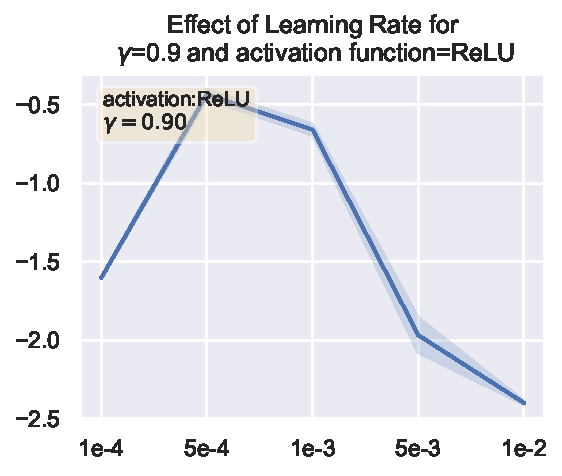
\includegraphics[width=0.325\textwidth]{SA_Gamma_0p9_ReLU.pdf}}
		\subfigure[\hlc{Discount factor $\gamma$=0.95}]{\label{fig_SA_G95_R}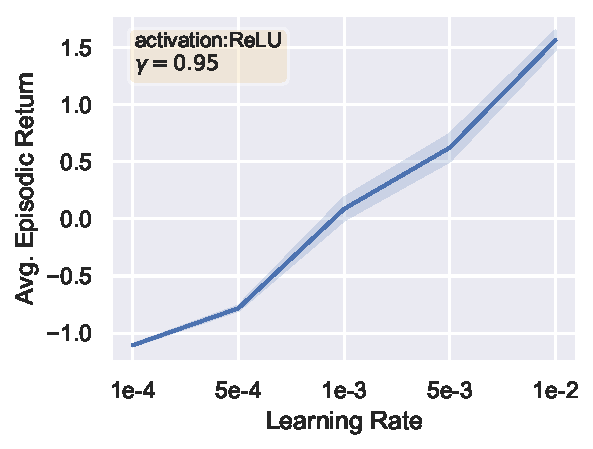
\includegraphics[width=0.325\textwidth]{SA_Gamma_0p95_ReLU.pdf}}
		\subfigure[\hlc{Discount factor $\gamma$=0.99}]{\label{fig_SA_G99_R}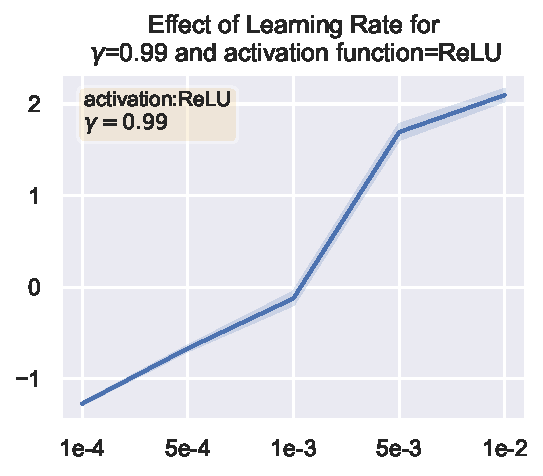
\includegraphics[width=0.325\textwidth]{SA_Gamma_0p99_ReLU.pdf}}		
		\caption{\hlc{Impact of changing learning rates and discount factor $\gamma$ for a REINFORCE policy network with ReLU activation.}}
		\label{fig_SA_LR_Relu}
	\end{figure}
	
	\begin{figure}[hbt!]
		\centering	
		\subfigure[\hlc{Discount factor $\gamma$=0.90}]{\label{fig_SA_G90_T}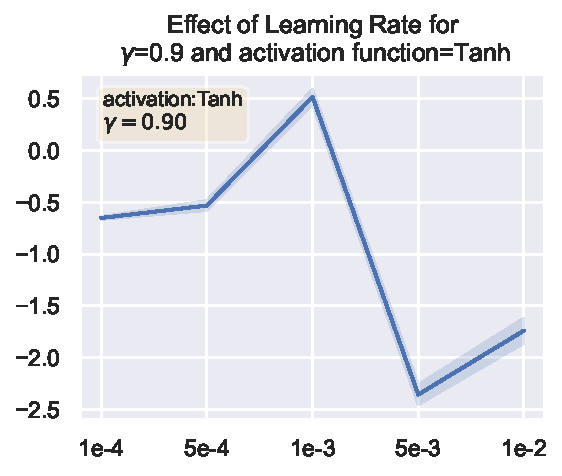
\includegraphics[width=0.325\textwidth]{SA_Gamma_0p9_Tanh.pdf}}
		\subfigure[\hlc{Discount factor $\gamma$=0.95}]{\label{fig_SA_G95_T}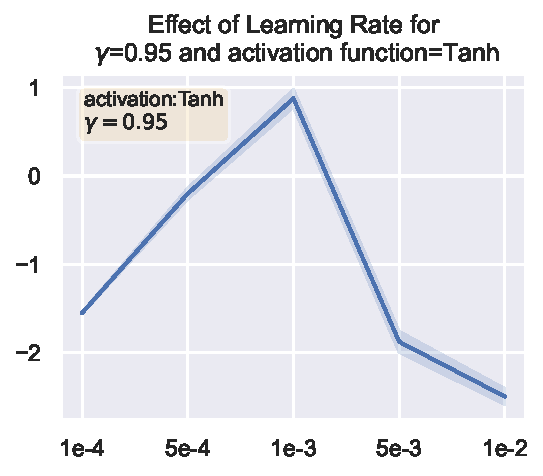
\includegraphics[width=0.325\textwidth]{SA_Gamma_0p95_Tanh.pdf}}
		\subfigure[\hlc{Discount factor $\gamma$=0.99}]{\label{fig_SA_G99_T}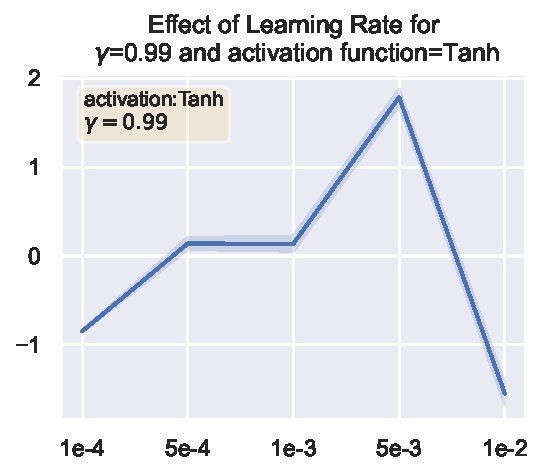
\includegraphics[width=0.325\textwidth]{SA_Gamma_0p99_Tanh.pdf}}		
		\caption{\hlc{Impact of changing learning rates and discount factor $\gamma$ for a REINFORCE policy network with Tanh activation.}}
		\label{fig_SA_LR_Tanh}
	\end{figure}
	
	\subsubsection*{\hlc{Impact of hyperparameter setting on training time}}
	\hlc{While REINFORCE performs reasonably well, it needs substantial time to train. To understand this better, we analyze it with respect to the same hyperparameter settings. In Fig.{\ref{fig_SA_TT_LR}}, we plot the time to train in panels of increasing learning rate, and in  Fig.{\ref{fig_SA_TT_G}}, we plot against panels of increasing {$\gamma$}. It is interesting to see that for Tanh based activation the training time increases for increasing learning rate and {$\gamma$}, whereas for ReLU it is relatively steady.}
	
	\begin{figure}[hbt!]
		\centering
		\subfigure[\hlc{Impact of learning rate}]{\label{fig_SA_TT_LR}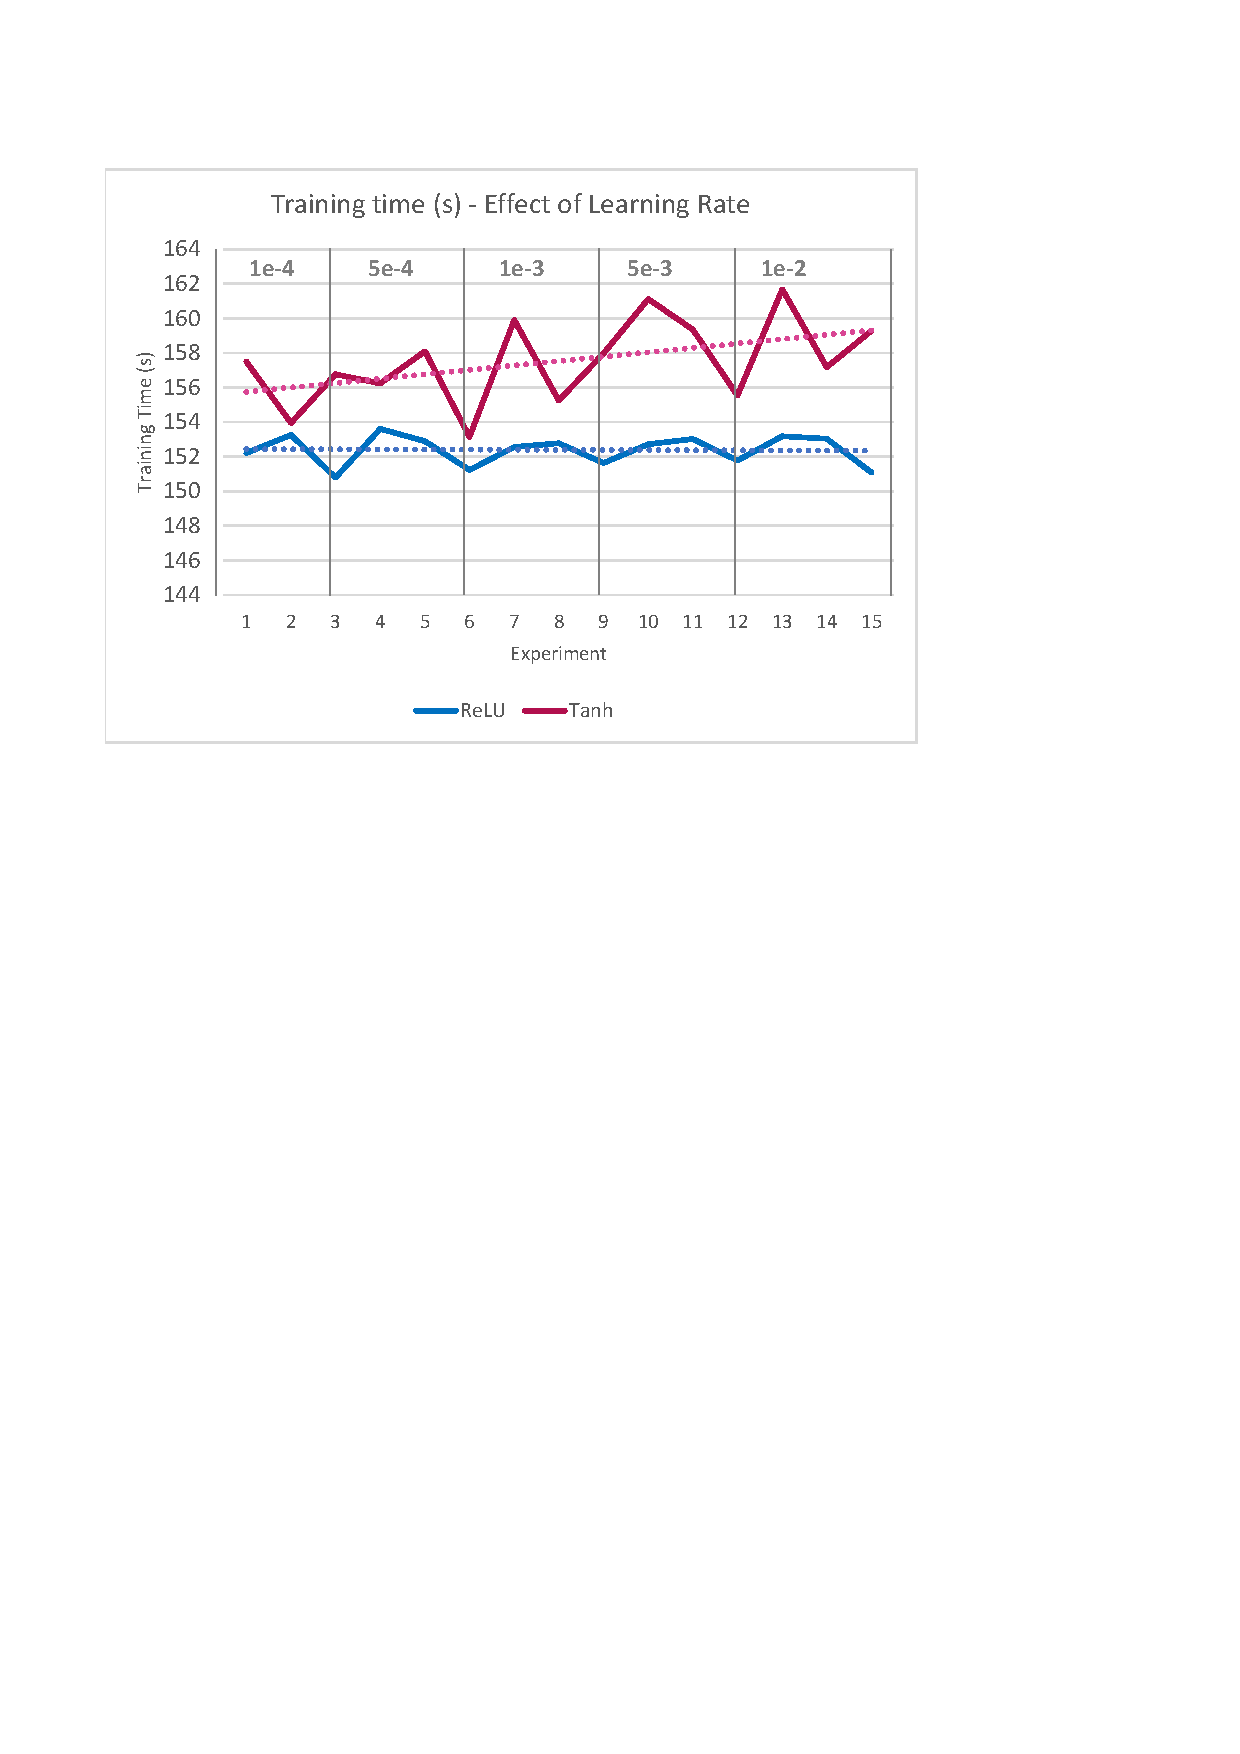
\includegraphics[clip, trim=1.75cm 17cm 5.25cm 2.75cm, width=0.475\textwidth]{TimeStudy_LR.pdf}}
		\subfigure[\hlc{Impact of discount factor $\gamma$}]{\label{fig_SA_TT_G}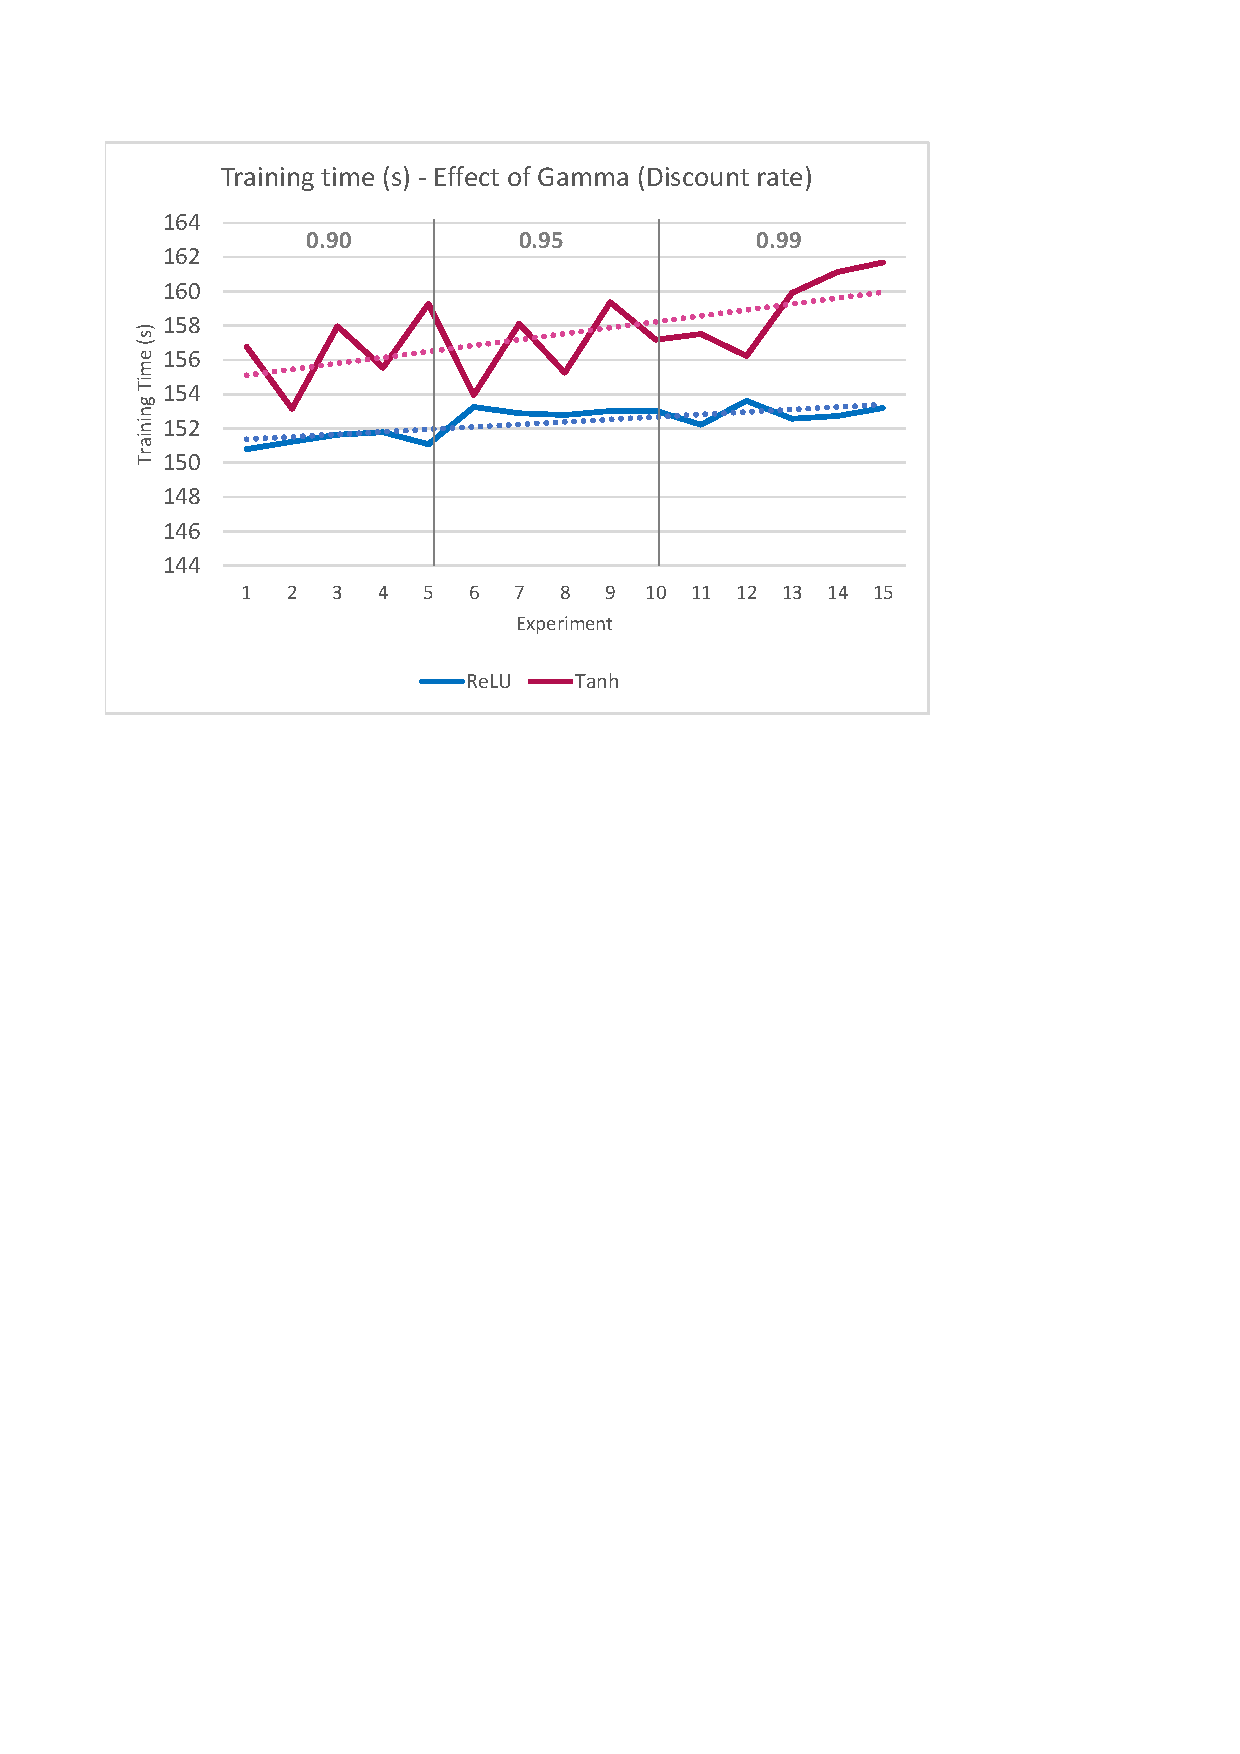
\includegraphics[clip, trim=1.75cm 17.5cm 5.25cm 2.15cm, width=0.475\textwidth]{TimeStudy_Gamma.pdf}}
		\caption{\hlc{Impact of learning rate and discount factor $\gamma$ on the time to train a REINFORCE model.}}
		\label{fig_SA_TrainingTime}
	\end{figure}
	
	\subsubsection*{\hlc{Compute cost of performance improvement}}
	\hlc{Increased training time generally translates to more intense use of compute resources and therefore increased cost. With Fig. {\ref{fig_SA_TrainingTime}} it is evident that the cost of compute is impacted primarily by the choice of activation function. One final question we seek to answer is; does this increase show any correlation with the model performance? Fig. {\ref{fig_perfcost}} shows that, for both the activation functions, generally increased time translates to increased performance; however due to REINFORCE's high variability, this is not a sharply defined pattern. Interestingly the ReLU, with significantly lower training cost compared to Tanh function, gives the best performing model (and as expected for higher training time {\textit{within}} the ReLU experiments).}
	
	\begin{figure}[hbt!]
		\centering
		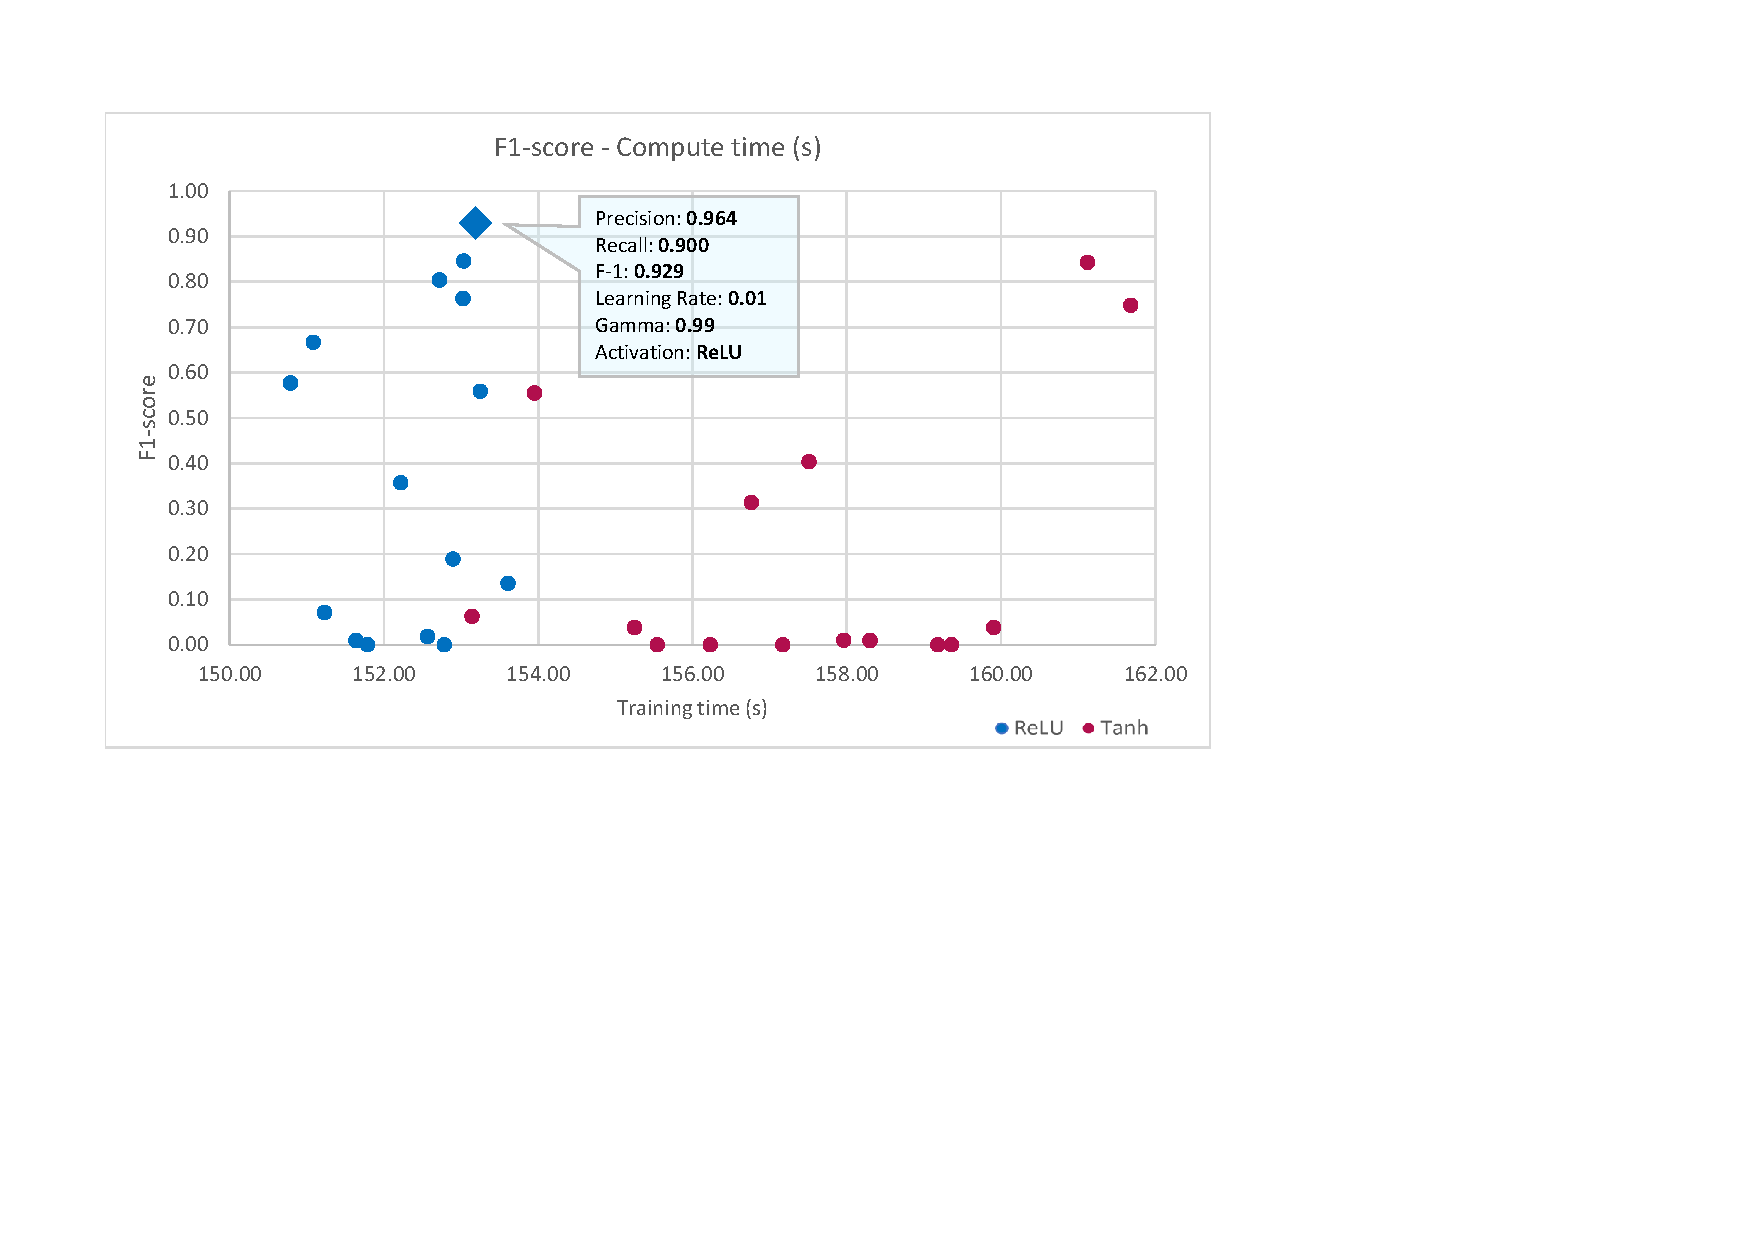
\includegraphics[clip, trim=1.75cm 8.2cm 8.75cm 1.75cm, width=0.7\textwidth]{TimeStudy_CostBenefitAnalysis.pdf}
		\caption{\hlc{The cost of performance improvement.}}
		\label{fig_perfcost}
	\end{figure}
	
	\section{Discussion}\label{sec_Discussion}
	%% $$$ glue
	\hlc{In Section} {\ref{sec_Results}} \hlc{we conducted a series of extensive experiments comparing REINFORCE with A2C, DQN, and PPO, with REINFORCE demonstrating significantly better performance than the other algorithms. As a closed-loop system, the performance of REINFORCE, like any RL system, will experience the effects of interaction of hyperparameters } \cite{autorl:parker2022}, \hlc{ therefore to better understand REINFORCE's performance we conducted a basic interaction and sensitivity analysis of hyperparameters, in Sec. {\ref{sec_SA}}. In this Discussion section, we first lay down views of researchers on the REINFORCE algorithm. We follow that by observations from our research, covering properties of this algorithm (both positive and limiting), aspects related to its architecture, training time, model size and cost effectiveness. We end the section with limitations of our research and potential areas for future research.}
	
	%% $$$ R2-2-13 Computational complexity
	\hlc{As a simple model-free RL algorithm, REINFORCE offers a derivative-free optimization of unconstrained problems.}{\cite{Matni2019}} \hlc{explains that, provided one can sample efficiently, REINFORCE can be used to solve essentially any problem!} The inventor of the REINFORCE algorithm, in his original paper \cite{REINFORCE-williams1992}, mentions the inability to predict the convergent and asymptotic properties of this algorithm using analytical means. The author mentions that \textit{simulation studies} are the primary source of understanding its behavior. 27 years later, \cite{peck2019} notes that rigorous convergence proofs are as of yet \textit{not} available for many algorithms based on REINFORCE and in their paper provide an intuition for convergence properties. This supports the extensive experimental studies on REINFORCE performed by \cite{zhang2021sample, zhang2021convergence, peck2019, duan2016benchmarking} as well our empirical research.  
	
	Both \cite{zhang2021convergence} and \cite{duan2016benchmarking} studied the behavior using multiple OpenAI Gym environments, while \cite{peck2019} provide empirical results using MuJuCo. \cite{duan2016benchmarking} observe that, despite its simplicity it is an effective algorithm in optimizing policies based on deep neural networks. On the other hand, their empirical study concluded that REINFORCE is occasionally trapped in premature convergence to local optima. REINFORCE suffers from high variance \cite{peck2019} and converges very slowly when it does. High variance implies that a large sample of environment interactions are needed to obtain a reasonable approximation of the actual gradient.
	
	\cite{zhang2021sample} provides the first known global convergence and sample efficiency results for the REINFORCE algorithm. Their study involved controlling the number of ``bad'' episodes as well as applying a ``doubling'' trick for studying the global convergence. Interestingly our training rounds resulted in multiple situations of ``zero'' performance (``bad'' episodes) for REINFORCE (18 instances) as also for Stable-Baseline's A2C implementation (12 instances); DQN and PPO did not show any occurrences.
	
	\hlc{Since RL algorithm implementations are} incredibly sensitive to hyperparameters and the neural network architectures they employ, the working implementations need several decisions to be made during high-, as well as low- level design; these strongly impact the performance, \cite{henderson2018deep, andrychowicz2021matters}. In fact the same algorithm could produce very different results depending on the code base one uses, \cite{henderson2018deep, SB3-paper}. \hlc{Our analysis in Sec. {\ref{sec_SA}} Fig. {\ref{fig_SA_LR_Relu}} indicates that, in general, higher model performance (average episodic rewards) is attained with higher discount factors $\gamma > 0.95$, learning rates in the range $5\times10^{-3}$ and $1\times10^{-2}$, and when the policy network is enabled by the ReLU activation function.}
	
	There could be \hlc{three} possible reasons for the positive performance demonstrated by REINFORCE. We used ReLU (rectified linear unit) as the activation function, while the other three algorithms used hyperbolic tangent (Tanh). \cite{henderson2018deep} studied four policy-gradient methods, including the PPO and TRPO, and observed that ReLU activation performs best. \hlc{Our study, Sec. {\ref{sec_SA}} Fig. {\ref{fig_SA_LR_Relu}} show higher average episodic rewards for ReLU based network and corroborates with the research findings of} {\cite{henderson2018deep}}. \hlc{The second reason is based on the observations by} \cite{duan2016benchmarking}. They observed that even with a small learning rate REINFORCE sometimes resulted in large changes to policy distribution, which possibly explains the fast convergence to local optima. On the other hand we used a larger learning rate (almost 50:1) and this could have assisted in reaching global optimas when it did. \hlc{In their survey of Auto RL, }\cite{autorl:parker2022}, \hlc{ states that the design of neural network architectures receives very little attention. Their survey concludes that there is a lack of conceptual understanding regarding architectural design choices and the benefits they offer. They state that most implementations use two or three hidden layers, similar to the algorithm implementations we studied in  (Sec. }{\ref{sec_architecture}}\hlc{). Our REINFORCE implementation was even simpler with just a single hidden layer and could be the third reason for the superior performance on simple environments.}
		
	%% $$$ R1-2 Strategies for reducing training time $
	\hlc{Training a REINFORCE algorithm requires more time. What strategies might help reducing this?} \cite{Lavet2016} \hlc{has conducted an extensive analysis on the interaction of $\gamma$ and the learning-rate. Lower values of $\gamma$ lead to faster convergence but by the very definition of {$\gamma$}, often result in myopic policies. Our study agrees with this, as seen in Fig. {\ref{fig_SA_TT_G}}, for both the activation functions. According to} \cite{Lavet2016} \hlc{one strategy for speeding up the learning process is to increase the discounting rate over time, rather than keeping it static. They further show that simultaneously decreasing the learning rate while increasing {$\gamma$} further reduces training time and thus improves learning speed. Our study points to one simple yet effective strategy of using ReLU activation layer for reducing training time, without sacrificing performance, Fig. {\ref{fig_perfcost}}}.
	
	%% $$$ R2-2 Runtime
	\hlc{We saw that the model sizes for all algorithms are under 140 KB. This implies that the runtime memory requirements are extremely small thus offering fast inferences. This suggests that such models can be used in embedded form on IoT devices and housed near the machines. This is a significant benefit for creating Industry 4.0 predictive maintenance solutions.} 
	
	\hlc{As a final point, we compare RL to the simpler ML methods, listed in Table {\ref{tbl_ml}}, used for a similar PdM problem. Supervised machine learning requires labeled data, RL on the other hand determines the right PdM action via trial and error. The manufacturing industry often lacks labeled fault data as reported by extremely recent surveys,} \cite{Leite2025, Hexagon2024}, \hlc{and this is one good reason for promoting RL. As can be seen in the existing literature, supervised ML, when labeled fault data is available, will outperform RL. Unlike the closed-loop RL, supervised ML is open-looped and the impact of hyperparameters is ascertainable and predictable and therefore are easier to tune,}  \cite{autorl:parker2022}. \hlc{In addition to being stable, they require far lower compute resources to train. It is therefore advisable to use ML in situations where good quality data is available.}
		
	%% $$$ R1-4 Limitations
	\subsection*{\hlc{Limitations and future scope for research}}
	
	\hlc{Our research carries limitations -- some due to the very design of our objective and some due to unavailability of more resources and time. These however offer opportunities for further research and increase the depth of this topic and provide more knowledge in the domain of AutoRL for predictive maintenance.}
	
	\begin{enumerate}
		\item \hlc{We used raw features, with no feature engineering.} This is in tune with the ``untuned'' algorithms concept. \hlc{However, this creats a \textit{possible} gap, where the more advanced models may demonstrate better performance}. With AutoRL one could automate such feature engineering techniques, followed by automated selection of significant features.
		\item \hlc{Advanced algorithms provide a richer set of hyperparameters and it is fair to assume that tuned versions of these algorithms will perform better than the na\"ive REINFORCE.}
		\item We assume that the human preventive maintenance policy, based on experience, is ideal. In practice this might not always be the case. \hlc{We had to use expert guidelines to decide the tool replacement wear thresholds} as these were not available for the PHM dataset.
	\end{enumerate}
	
	\hlc{\textbf{Avenues for future research}: Our research covers single-agent RL. Multi-agent and multi-objective RL can solve more complex problems and are areas we plan to research in the near future. Offline RL (also called Batch RL) is a paradigm where offline data in the form of previously collected data such as expert demonstrations and experiments, offer a path to generalize agents to a real world environment. No environment interaction is required in offline RL. Offline RL is suitable for the PdM domain and as such recommended for future research.}
	
	\section{Conclusion}\label{sec_Conclusion}
	The REINFORCE is a simple algorithm and our na\"ive implementation can be improved drastically, for example with the implementation of a baseline to reduce variance. We evaluated the REINFORCE along with industry grade implementations of more advanced algorithms, DQN, A2C and PPO, over 15 environment variants (simulated and real data). Despite its simplicity, known variance and convergence issues, it performed surprisingly well, as observed through numerical results, plots and statistical tests. \hlc{The hyperparameter interaction study provided insights into the impact on performance, of the two standard hyperparameters studied in the RL domain, i.e., the learning rate and the discount factor $\gamma$. Additionally, we studied the impact of the two most common activation functions used for implementing RL algorithms i.e. ReLU and Tanh. All this has surely created a valuable knowledge resource for the simple, often neglected, REINFORCE algorithm.}
	
	Implementing robust RL algorithms is complex and \cite{SB3-paper} puts this beautifully, mentioning how small implementation details can significantly impact performance \textit{``that is often greater than the difference between the algorithms themselves''}. 
	
	We hope our research contributes to empirical evidence related to the application of REINFORCE to predictive maintenance. This contribution aims to play a vital role in advancing the prospects of automated reinforcement learning i.e. AutoRL to Industry 4.0 revolution.
	
	\backmatter
	
	%\bmhead{Supplementary information}
	
	\bmhead{Acknowledgements}
	\hlc{We would like to sincerely thank the anonymous reviewers of this research article. They highlighted some deeper analysis that we performed adding significantly to the empirical richness of this research.}
	
	\section*{Declarations}
	
	\subsection*{Funding}
	None.
	\subsection*{Conflict of interest/Competing interests}
	The authors report there are no competing interests to declare.
	
	\subsection*{Ethics approval and consent to participate}
	Not applicable.
	
	\subsection*{Consent for publication}
	All listed authors grant permission for publication.
	
	\subsection*{Data availability}
	The data used for model training and validation is from \cite{PHM-dataset} and publicly available at \href{https://doi.org/10.21227/jdxd-yy51}{IEEE\textit{DataPort}}. 
	
	\subsection*{Materials availability}
	\subsection*{Code availability}
	Will be available on request, via a GitHub link.
	\subsection*{Author contribution}
	%Conceptualization, R.S.; methodology, R.S.; software, R.S.; validation, S.K., S.P. and A.B.; formal analysis, R.S.; resources, S.K. and S.P.; data curation, R.S.; writing---original draft preparation, R.S.; writing---review and editing, S.K, S.P. and K.K.; supervision, S.K. and S.P.; project administration, S.K. and A.B.; funding acquisition, K.K. and S.A. All authors have read and agreed to the published version of the manuscript.
	
	\bigskip
	\bigskip
	%\clearpage
	\begin{appendices}
		\setcounter{table}{0}
		\renewcommand\theHtable{Appendix.\thetable}
		\setcounter{figure}{0}
		\renewcommand\theHfigure{Appendix.\thefigure}
		
		\section{Detailed results}\label{apx}
		The Appendix contains detailed tabulated results as well as validation plots.
		\begin{table}[!h]
			\rowspace{1.6}
			\caption{Reference table for results.}\label{tbl_apx_results}
			{\begin{tabular}{R{0.25cm} L{11.5cm} L{3cm}}
					\arrayrulecolor{black!40}\toprule 			
					& Item & Reference\\ \midrule
					
					%\rowcolor{ltgray} & \textbf{Detailed Results} - Appendix \ref{apx} & \\
					1 & Complete detailed results -- All 15 environments, averaged over 10 rounds & Table \ref{tbl_DetailedMetrics}\\\ltmidrule
					
					2 & Super Models -- Best model, \textit{details} of all 15 environments & Table \ref{tbl_SuperModelsDetailedMetrics}\\\ltmidrule
					
					3 & Stability behavior plots over 10 rounds, Precision, Recall and F1\\
					& \quad\quad Overall (all variants)  & Fig. \ref{fig_tr-overall}\\
					& \quad\quad Simulated state & Fig. \ref{fig_tr-sim-env}\\
					& \quad\quad Simple univariate state & Fig. \ref{fig_tr-ss-env}\\
					& \quad\quad Complex multivariate state & Fig. \ref{fig_tr-ms-env}\\
					\bottomrule
			\end{tabular}}
		\end{table}
		
		%\setcounter{table}{1}
		\begin{sidewaystable}
			\caption{Model performance comparison all variants of the environments, over 10 rounds of training. Maximum values indicated in \textcolor{dblue}{blue}.}\label{tbl_DetailedMetrics}
			{\begin{tabular}{@{}l| rrrr @{}c| rrrr @{}c| rrrr @{}c| rrrr@{}} \arrayrulecolor{black!40}\toprule
					& \multicolumn{4}{c}{\textbf{REINFORCE}} & & \multicolumn{4}{c}{A2C} &
					& \multicolumn{4}{c}{DQN} & & \multicolumn{4}{c}{PPO} \\
					\cmidrule{2-5} \cmidrule{7-10} \cmidrule{12-15} \cmidrule{17-20}
					Environment &Prec. &Recall &F1 &F$_\beta$0.5 & &Prec. &Recall &F1 &F$_\beta$0.5 & &Prec. &Recall &F1 &F$_\beta$0.5 & &Prec. &Recall &F1 &F$_\beta$0.5\\ \midrule
					Simulated  - No noise &\textcolor{dblue}{0.842} &\textcolor{dblue}{0.878} &\textcolor{dblue}{0.838} & \textcolor{dblue}{0.834} & & 0.424 &0.451 &0.423 &0.421 & &0.426 &0.674 &0.471 &0.410 & &0.504 &0.200 &0.271&0.360\\
					Simulated  - Low noise &\textcolor{dblue}{0.777} &\textcolor{dblue}{0.929} &\textcolor{dblue}{0.834} & \textcolor{dblue}{0.796} & & 0.465 &0.423 &0.409 &0.427 & &0.421 &0.338 &0.270 &0.283 & &0.482 &0.236 &0.296&0.369\\
					Simulated  - High noise &\textcolor{dblue}{0.798} &\textcolor{dblue}{0.940} &\textcolor{dblue}{0.851} & \textcolor{dblue}{0.816} & & 0.358 &0.281 &0.256 &0.272 & &0.447 &0.519 &0.380 &0.360 & &0.514 &0.207 &0.286&0.382\\ \midrule
					
					PHM C01 SS - No noise &0.478 &0.363 &0.400 & 0.439 & & \textcolor{dblue}{0.501} &0.500 &0.493 &\textcolor{dblue}{0.496} & &0.472 &\textcolor{dblue}{0.807} &\textcolor{dblue}{0.568} &0.490 & &0.440 &0.417 &0.387&0.395\\
					PHM C01 SS - Low noise &0.507 &0.311 &0.332 & 0.383 & & \textcolor{dblue}{0.503} &\textcolor{dblue}{0.598} &\textcolor{dblue}{0.535} &\textcolor{dblue}{0.513} & &0.393 &0.502 &0.351 &0.317 & &0.522 &0.338 &0.388&0.448\\
					PHM C01 SS - High noise &\textcolor{dblue}{0.693} &\textcolor{dblue}{0.562} &\textcolor{dblue}{0.579} & \textcolor{dblue}{0.623} & & 0.266 &0.282 &0.267 &0.262 & &0.458 &0.525 &0.400 &0.384 & &0.456 &0.369 &0.372&0.400\\ \hdashline
					
					PHM C04 SS - No noise &\textcolor{dblue}{0.751} &\textcolor{dblue}{0.878} &\textcolor{dblue}{0.784} & \textcolor{dblue}{0.757} & & 0.487 &0.442 &0.449 &0.463 & &0.439 &0.684 &0.472 &0.411 & &0.500 &0.510 &0.469&0.473\\
					PHM C04 SS - Low noise &\textcolor{dblue}{0.662} &\textcolor{dblue}{0.756} &\textcolor{dblue}{0.672} & \textcolor{dblue}{0.657} & & 0.409 &0.455 &0.428 &0.416 & &0.411 &0.500 &0.370 &0.341 & &0.488 &0.280 &0.324&0.386\\
					PHM C04 SS - High noise &\textcolor{dblue}{0.611} &\textcolor{dblue}{0.713} &\textcolor{dblue}{0.620} & \textcolor{dblue}{0.598} & & 0.518 &0.607 &0.552 &0.530 & &0.358 &0.451 &0.325 &0.294 & &0.428 &0.262 &0.286&0.333\\ \hdashline
					
					PHM C06 SS - No noise &\textcolor{dblue}{0.830} &\textcolor{dblue}{0.726} &\textcolor{dblue}{0.754} & \textcolor{dblue}{0.792} & & 0.517 &0.509 &0.507 &0.511 & &0.360 &0.309 &0.256 &0.258 & &0.409 &0.248 &0.275&0.321\\
					PHM C06 SS - Low noise &0.205 &0.279 &0.228 & 0.212 & & \textcolor{dblue}{0.510} &\textcolor{dblue}{0.577} &\textcolor{dblue}{0.530} &\textcolor{dblue}{0.516} & &0.434 &0.266 &0.266 &0.296 & &0.417 &0.181 &0.232&0.294\\
					PHM C06 SS - High noise &\textcolor{dblue}{0.709} &\textcolor{dblue}{0.843} &\textcolor{dblue}{0.759 }& \textcolor{dblue}{0.726} & & 0.316 &0.324 &0.311 &0.308 & &0.449 &0.518 &0.400 &0.375 & &0.388 &0.222 &0.265&0.317\\ \midrule
					
					PHM C01 MS - No noise &\textcolor{dblue}{0.835} &\textcolor{dblue}{0.652} &\textcolor{dblue}{0.656} & \textcolor{dblue}{0.716} & & 0.461 &0.444 &0.397 &0.404 & &0.384 &0.558 &0.393 &0.348 & &0.513 &0.383 &0.416&0.460\\
					PHM C04 MS - No noise &\textcolor{dblue}{0.739} &0.255 &0.359 & \textcolor{dblue}{0.494} & & 0.498 &\textcolor{dblue}{0.589 }&\textcolor{dblue}{0.490} &0.470 & &0.323 &0.209 &0.160 &0.168 & &0.499 &0.393 &0.421&0.457\\
					PHM C06 MS - No noise &\textcolor{dblue}{0.864} &0.356 &0.469 & \textcolor{dblue}{0.616} & & 0.501 &\textcolor{dblue}{0.713} &\textcolor{dblue}{0.578} &0.527 & &0.489 &0.705 &0.529 &0.479 & &0.523 &0.488 &0.485&0.498\\
					
					\bottomrule
			\end{tabular}}
		\end{sidewaystable}
		
		%\setcounter{table}{1}
		\begin{sidewaystable}
			\caption{Super Models: Best models selected over 10 rounds of training. Maximum performance values indicated in \textcolor{dblue}{blue}.}\label{tbl_SuperModelsDetailedMetrics}
			{\begin{tabular}{@{}l| rrrr @{}c| rrrr @{}c| rrrr @{}c| rrrr@{}} \arrayrulecolor{black!40}\toprule
					& \multicolumn{4}{c}{\textbf{REINFORCE}} & & \multicolumn{4}{c}{A2C} &
					& \multicolumn{4}{c}{DQN} & & \multicolumn{4}{c}{PPO} \\
					\cmidrule{2-5} \cmidrule{7-10} \cmidrule{12-15} \cmidrule{17-20}
					Environment &Prec. &Recall &F1 &F$_\beta$0.5 & &Prec. &Recall &F1 &F$_\beta$0.5 & &Prec. &Recall &F1 &F$_\beta$0.5 & &Prec. &Recall &F1 &F$_\beta$0.5\\ \midrule
					Simulated  - No noise &\textcolor{dblue}{0.897} &0.960 &\textcolor{dblue}{0.926} & \textcolor{dblue}{0.908} & & 0.500 &\textcolor{dblue}{1.000} &0.667 &0.556 & &0.505 &0.980 &0.667 &0.560 & &0.669 &0.430 &0.518&0.597\\
					Simulated  - Low noise &\textcolor{dblue}{0.960} &0.945 &\textcolor{dblue}{0.952} & \textcolor{dblue}{0.957} & & 0.516 &\textcolor{dblue}{1.000} &0.680 &0.571 & &0.500 &0.980 &0.662 &0.554 & &0.633 &0.460 &0.530&0.586\\
					Simulated  - High noise &\textcolor{dblue}{0.922} &0.990 &\textcolor{dblue}{0.955} & \textcolor{dblue}{0.935} & & 0.503 &\textcolor{dblue}{1.000} &0.669 &0.558 & &0.504 &0.990 &0.668 &0.559 & &0.569 &0.355 &0.434&0.505\\\midrule
					
					PHM C01 SS - No noise &\textcolor{dblue}{0.889} &0.995 &\textcolor{dblue}{0.939} & \textcolor{dblue}{0.908} & & 0.586 &0.625 &0.603 &0.592 & &0.647 &0.970 &0.776 &0.693 & &0.543 &\textcolor{dblue}{1.000} &0.703&0.597\\
					PHM C01 SS - Low noise &\textcolor{dblue}{0.988} &0.765 &\textcolor{dblue}{0.861} & \textcolor{dblue}{0.932} & & 0.499 &0.995 &0.664 &0.554 & &0.504 &\textcolor{dblue}{0.990} &0.668 &0.559 & &0.623 &0.740 &0.675&0.643\\
					PHM C01 SS - High noise &\textcolor{dblue}{0.850} &0.970 &\textcolor{dblue}{0.905} & \textcolor{dblue}{0.871} & & 0.521 &0.680 &0.588 &0.546 & &0.505 &\textcolor{dblue}{0.985} &0.668 &0.560 & &0.520 &0.725 &0.604&0.551\\\hdashline
					
					PHM C04 SS - No noise &\textcolor{dblue}{0.811} &\textcolor{dblue}{1.000} &\textcolor{dblue}{0.895} & \textcolor{dblue}{0.842} & & 0.536 &0.645 &0.583 &0.554 & &0.501 &0.965 &0.660 &0.554 & &0.579 &0.895 &0.702&0.622\\
					PHM C04 SS - Low noise &\textcolor{dblue}{0.798} &0.980 &\textcolor{dblue}{0.879} & \textcolor{dblue}{0.829} & & 0.556 &0.665 &0.603 &0.573 & &0.734 &\textcolor{dblue}{0.990} &0.843 &0.774 & &0.546 &0.660 &0.596&0.565\\
					PHM C04 SS - High noise &\textcolor{dblue}{0.708} &0.840 &\textcolor{dblue}{0.767} & \textcolor{dblue}{0.730} & & 0.521 &0.835 &0.641 &0.563 & &0.511 &\textcolor{dblue}{0.985} &0.672 &0.565 & &0.517 &0.820 &0.633&0.558\\\hdashline
					
					PHM C06 SS - No noise &\textcolor{dblue}{1.000} &\textcolor{dblue}{0.895} &\textcolor{dblue}{0.944} & \textcolor{dblue}{0.977} & & 0.520 &0.680 &0.587 &0.545 & &0.935 &0.975 &0.954 &0.942 & &0.587 &0.650 &0.615&0.597\\
					PHM C06 SS - Low noise &\textcolor{dblue}{0.943} &0.795 &\textcolor{dblue}{0.861} & \textcolor{dblue}{0.908} & & 0.501 &\textcolor{dblue}{1.000} &0.668 &0.557 & &0.961 &0.725 &0.826 &0.901 & &0.552 &0.370 &0.438&0.497\\
					PHM C06 SS - High noise &0.821 &0.845 &0.831 & 0.825 & & 0.540 &0.755 &0.628 &0.572 & &\textcolor{dblue}{0.980} &\textcolor{dblue}{0.960}&\textcolor{dblue}{0.969} &\textcolor{dblue}{0.976} & &0.521 &0.615 &0.564&0.537\\\midrule
					
					PHM C01 MS - No noise &\textcolor{dblue}{0.827} &0.995 &\textcolor{dblue}{0.903} & \textcolor{dblue}{0.856} & & 0.500 &\textcolor{dblue}{1.000} &0.667 &0.556 & &0.505 &0.985 &0.668 &0.560 & &0.512 &0.595 &0.549&0.526\\
					PHM C04 MS - No noise &\textcolor{dblue}{0.910}&0.425 &0.577 & \textcolor{dblue}{0.738} & & 0.500 &\textcolor{dblue}{1.000} &\textcolor{dblue}{0.667} &0.556 & &0.501 &0.975 &0.662 &0.555 & &0.501 &0.635 &0.558&0.522\\
					PHM C06 MS - No noise &\textcolor{dblue}{0.934} &0.865 &\textcolor{dblue}{0.896} & \textcolor{dblue}{0.918} & & 0.500 &\textcolor{dblue}{1.000} &0.667 &0.556 & &0.969 &0.600 &0.741 &0.863 & &0.497 &0.690 &0.577&0.526\\			
					\bottomrule
				\end{tabular}			
			}
		\end{sidewaystable}
		
		\begin{figure}
			\centering	
			\subfigure[Precision]{\label{fig_tr-ovr-pr}\includegraphics[width=\linewidth]{Overall_Pr.pdf}}
			\subfigure[Recall]{\label{fig_tr-ovr-rc}\includegraphics[width=\linewidth]{Overall_Rc.pdf}}
			\subfigure[F1-score]{\label{fig_tr-ovr-f}\includegraphics[width=\linewidth]{Overall_F1.pdf}}	
			\caption{Overall performance -- Average over 10 modelsOverall performance -- Average over 10 models}
			\label{fig_tr-overall}
		\end{figure}
		
		\begin{figure}
			\centering	
			\subfigure[Precision]{\label{fig_tr-sim-pr}\includegraphics[width=\linewidth]{Simulated_Pr.pdf}}
			\subfigure[Recall]{\label{fig_tr-sim-rc}\includegraphics[width=\linewidth]{Simulated_Rc.pdf}}
			\subfigure[F1-score]{\label{fig_tr-sim-f}\includegraphics[width=\linewidth]{Simulated_F1.pdf}}	
			\caption{Simulated environment -- Average over 10 models}
			\label{fig_tr-sim-env}
		\end{figure}
		
		\begin{figure}
			\centering	
			\subfigure[Precision]{\label{fig_tr-ss-pr}\includegraphics[width=\linewidth]{Singevariable_Pr.pdf}}
			\subfigure[Recall]{\label{fig_tr-ss-rc}\includegraphics[width=\linewidth]{Singevariable_Rc.pdf}}
			\subfigure[F1-score]{\label{fig_tr-ss-f}\includegraphics[width=\linewidth]{Singevariable_F1.pdf}}	
			\caption{Univariate environment -- Average over 10 models}
			\label{fig_tr-ss-env}
		\end{figure}
		
		\begin{figure}
			\centering	
			\subfigure[Precision]{\label{fig_tr-ms-pr}\includegraphics[width=\linewidth]{Multivariate_Pr.pdf}}
			\subfigure[Recall]{\label{fig_tr-ms-rc}\includegraphics[width=\linewidth]{Multivariate_Rc.pdf}}
			\subfigure[F1-score]{\label{fig_tr-ms-f}\includegraphics[width=\linewidth]{Multivariate_F1.pdf}}	
			\caption{Multivariate environment -- Average over 10 models}
			\label{fig_tr-ms-env}
		\end{figure}
		
		
	\end{appendices}
	\clearpage
	\bibliography{bibliography}
\end{document}
